\newpage
\chapter{HASIL DAN PEMBAHASAN} \label{Bab IV}

\section{Pendahuluan}

Bab ini menyajikan hasil eksperimen \textit{fine-tuning} model Whisper Base pada bahasa Minangkabau menggunakan dua strategi: \textit{Freeze Encoder} dan \textit{Low-Rank Adaptation} (LoRA) \cite{hu2022lora}. Kedua strategi dievaluasi menggunakan metodologi 5-\textit{fold cross-validation} \cite{kohavi1995crossvalidation} pada dataset yang sama (156 file audio, $\sim$1,3 jam) untuk memastikan perbandingan yang adil. Bab ini dimulai dengan hasil masing-masing strategi, dilanjutkan dengan analisis perbandingan dan pembahasan.

%% ====================================================================
%% SECTION: HASIL FREEZE ENCODER
%% ====================================================================
\section{Hasil Strategi Freeze Encoder} \label{IV.FreezeEncoder}

\subsection{Perbandingan Eksperimen Freeze Encoder}

Selama proses penelitian, dilakukan lima kali percobaan pelatihan (\textit{run}) dengan strategi \textit{Freeze Encoder} untuk menemukan konfigurasi optimal. Tabel~\ref{tab:fe_run_configs} merangkum konfigurasi yang digunakan pada setiap percobaan, dan Tabel~\ref{tab:fe_run_comparison} merangkum hasilnya.

\begin{table}[H]
\centering
\caption{Konfigurasi Hyperparameter Lima Percobaan Freeze Encoder}
\label{tab:fe_run_configs}
\resizebox{\textwidth}{!}{%
\begin{tabular}{|l|c|c|c|c|c|}
\hline
\textbf{Parameter} & \textbf{Run 1} & \textbf{Run 2} & \textbf{Run 3} & \textbf{Run 4} & \textbf{Run 5} \\
 & \textbf{(22 Jan, 16:00)} & \textbf{(22 Jan, 16:57)} & \textbf{(22 Jan, 17:32)} & \textbf{(8 Feb, 14:51)} & \textbf{(12 Feb, 06:00)} \\
\hline
\hline
\multicolumn{6}{|c|}{\textbf{Konfigurasi Training}} \\
\hline
Learning Rate & 5$\times$10\textsuperscript{-6} & 1$\times$10\textsuperscript{-5} & 1$\times$10\textsuperscript{-5} & 1$\times$10\textsuperscript{-5} & 1$\times$10\textsuperscript{-5} \\
\hline
Batch Size & 16 & 16 & 16 & 32 & 32 \\
\hline
Gradient Accumulation & 2 & 2 & 2 & 1 & 1 \\
\hline
Effective Batch Size & 32 & 32 & 32 & 32 & 32 \\
\hline
Max Steps & 200 & 200 & 200 & 200 & 120 \\
\hline
Warmup Ratio & 0,2 & 0,2 & 0,2 & 0,2 & 0,2 \\
\hline
Weight Decay & 0,2 & 0,2 & 0,2 & 0,1 & 0,1 \\
\hline
Label Smoothing & --- & --- & --- & --- & 0,1 \\
\hline
LR Scheduler & Cosine & Cosine & Cosine & Cosine & Cosine \\
\hline
\hline
\multicolumn{6}{|c|}{\textbf{Konfigurasi Dropout Model}} \\
\hline
Decoder Dropout & 0,3 & 0,3 & 0,3 & 0,3 & 0,2 \\
\hline
Attention Dropout & 0,2 & 0,2 & 0,2 & 0,2 & 0,15 \\
\hline
Activation Dropout & 0,2 & 0,2 & 0,2 & 0,2 & 0,15 \\
\hline
\hline
\multicolumn{6}{|c|}{\textbf{Decoding}} \\
\hline
Beam Width & 1 (greedy) & 1 (greedy) & 1 (greedy) & 5 & 5 \\
\hline
\end{tabular}%
}
\end{table}

\begin{table}[H]
\centering
\caption{Perbandingan Hasil Lima Percobaan Freeze Encoder}
\label{tab:fe_run_comparison}
\resizebox{\textwidth}{!}{%
\begin{tabular}{|c|c|c|c|c|c|c|c|}
\hline
\textbf{Run} & \textbf{Learning Rate} & \textbf{Batch Size} & \textbf{Weight Decay} & \textbf{Label Smooth.} & \textbf{Beam} & \textbf{Mean WER (\%)} & \textbf{Mean CER (\%)} \\
\hline
1 (22 Jan, 16:00) & 5$\times$10\textsuperscript{-6} & 16$\times$2 & 0,2 & --- & 1 & 25,07 $\pm$ 2,86 & 5,60 $\pm$ 0,59 \\
\hline
2 (22 Jan, 16:57) & 1$\times$10\textsuperscript{-5} & 16$\times$2 & 0,2 & --- & 1 & 22,34 $\pm$ 1,89 & 4,93 $\pm$ 0,55 \\
\hline
3 (22 Jan, 17:32) & 1$\times$10\textsuperscript{-5} & 16$\times$2 & 0,2 & --- & 1 & 22,95 $\pm$ 2,70 & 5,52 $\pm$ 0,77 \\
\hline
4 (8 Feb, 14:51) & 1$\times$10\textsuperscript{-5} & 32$\times$1 & 0,1 & --- & 5 & 19,92 $\pm$ 2,42 & 4,53 $\pm$ 0,65 \\
\hline
\textbf{5 (12 Feb, 06:00)} & \textbf{1$\times$10\textsuperscript{-5}} & \textbf{32$\times$1} & \textbf{0,1} & \textbf{0,1} & \textbf{5} & \textbf{20,34 $\pm$ 2,41} & \textbf{4,46 $\pm$ 0,50} \\
\hline
\end{tabular}%
}
\end{table}

Run 5 mencapai performa terbaik dengan rata-rata WER \textbf{20,34\%} dan CER \textbf{4,46\%}. Meskipun WER rata-rata Run 5 sedikit lebih tinggi dibandingkan Run 4 (20,34\% vs 19,92\%), Run 5 mencapai CER yang lebih rendah (4,46\% vs 4,53\%) dan standar deviasi WER yang lebih kecil (2,41\% vs 2,42\%). Berdasarkan analisis konfigurasi pada Tabel~\ref{tab:fe_run_configs}, evolusi percobaan menunjukkan beberapa temuan:

\begin{enumerate}
    \item \textbf{Run 1 vs Run 2} (pengaruh \textit{learning rate}): Peningkatan \textit{learning rate} dari 5$\times$10\textsuperscript{-6} ke 1$\times$10\textsuperscript{-5} menghasilkan penurunan WER signifikan (25,07\% $\rightarrow$ 22,34\%), menunjukkan bahwa \textit{learning rate} awal terlalu kecil untuk konvergensi yang efektif.
    
    \item \textbf{Run 2 vs Run 3} (reproduktibilitas): Kedua run menggunakan konfigurasi identik namun menghasilkan WER yang berbeda (22,34\% vs 22,95\%), menunjukkan variabilitas dari \textit{stochastic training} yang perlu diperhatikan dalam interpretasi hasil.
    
    \item \textbf{Run 4} (optimasi multi-faktor): Penurunan \textit{weight decay} dari 0,2 ke 0,1, peningkatan \textit{batch size} fisik dari 16 menjadi 32, dan penggunaan \textit{beam search} (\textit{width}=5) menghasilkan penurunan WER signifikan (22,34\% $\rightarrow$ 19,92\%) \cite{radford2023whisper}.
    
    \item \textbf{Run 5} (\textit{label smoothing} + penyesuaian regularisasi): Penambahan \textit{label smoothing} 0,1 \cite{szegedy2016rethinking} dengan penurunan \textit{dropout} (0,2/0,15/0,15 vs 0,3/0,2/0,2 pada Run 4) dan pengurangan \textit{max steps} (120 vs 200) menghasilkan model dengan CER lebih rendah (4,46\% vs 4,53\%) dan konsistensi yang lebih baik (std WER 2,41\% vs 2,42\%). \textit{Label smoothing} membagi beban regularisasi dengan \textit{dropout}, sehingga \textit{dropout} dapat diturunkan tanpa meningkatkan risiko \textit{overfitting}.
\end{enumerate}

Analisis selanjutnya menggunakan hasil dari \textbf{Run 5} (run\_20260212\_060037) karena menggunakan konfigurasi regularisasi terlengkap dan menunjukkan keseimbangan terbaik antara performa dan konsistensi.

\subsection{Hasil Cross-Validation Freeze Encoder}

Tabel~\ref{tab:fe_cv_results} menunjukkan hasil evaluasi 5-\textit{fold cross-validation} untuk strategi \textit{Freeze Encoder}.

\begin{table}[H]
\centering
\caption{Hasil 5-Fold Cross-Validation Strategi Freeze Encoder}
\label{tab:fe_cv_results}
\begin{tabular}{|c|c|c|c|c|c|}
\hline
\textbf{Fold} & \textbf{Train} & \textbf{Eval} & \textbf{WER (\%)} & \textbf{CER (\%)} & \textbf{Steps} \\
\hline
0 & 124 & 32 & 20,36 & 4,28 & 96 \\
\hline
1 & 125 & 31 & 19,76 & 4,58 & 116 \\
\hline
2 & 125 & 31 & \textbf{16,81} & \textbf{3,60} & 108 \\
\hline
3 & 125 & 31 & 24,37 & 4,90 & 120 \\
\hline
4 & 125 & 31 & 20,41 & 4,96 & 116 \\
\hline
\hline
\textbf{Mean} & \textbf{125} & \textbf{31} & \textbf{20,34 $\pm$ 2,41} & \textbf{4,46 $\pm$ 0,50} & \textbf{111,2} \\
\hline
\end{tabular}
\end{table}

\textbf{Catatan Metodologi}: \textit{Evaluation set} juga digunakan untuk \textit{early stopping} selama training (setiap 4 steps). Pendekatan ini merupakan \textit{pragmatic trade-off} yang umum dalam riset \textit{extremely low-resource}, di mana memisahkan \textit{validation set} akan mengurangi data training secara signifikan. Metrik yang dilaporkan berasal dari \textit{best checkpoint} dan berpotensi sedikit optimistis. Catatan metodologi ini berlaku juga untuk strategi LoRA.

\textit{Fold}~2 mencapai performa terbaik (WER 16,81\%, CER 3,60\%), sedangkan \textit{Fold}~3 menunjukkan WER tertinggi (24,37\%). Rentang WER antar-\textit{fold} sebesar 7,56 poin persentase mencerminkan sensitivitas model terhadap pembagian data pada dataset kecil.

\subsection{Konvergensi Training Freeze Encoder}

Gambar~\ref{fig:fe_training_loss} menampilkan kurva \textit{training loss} untuk kelima \textit{fold} pada strategi \textit{Freeze Encoder}.

\begin{figure}[H]
\centering
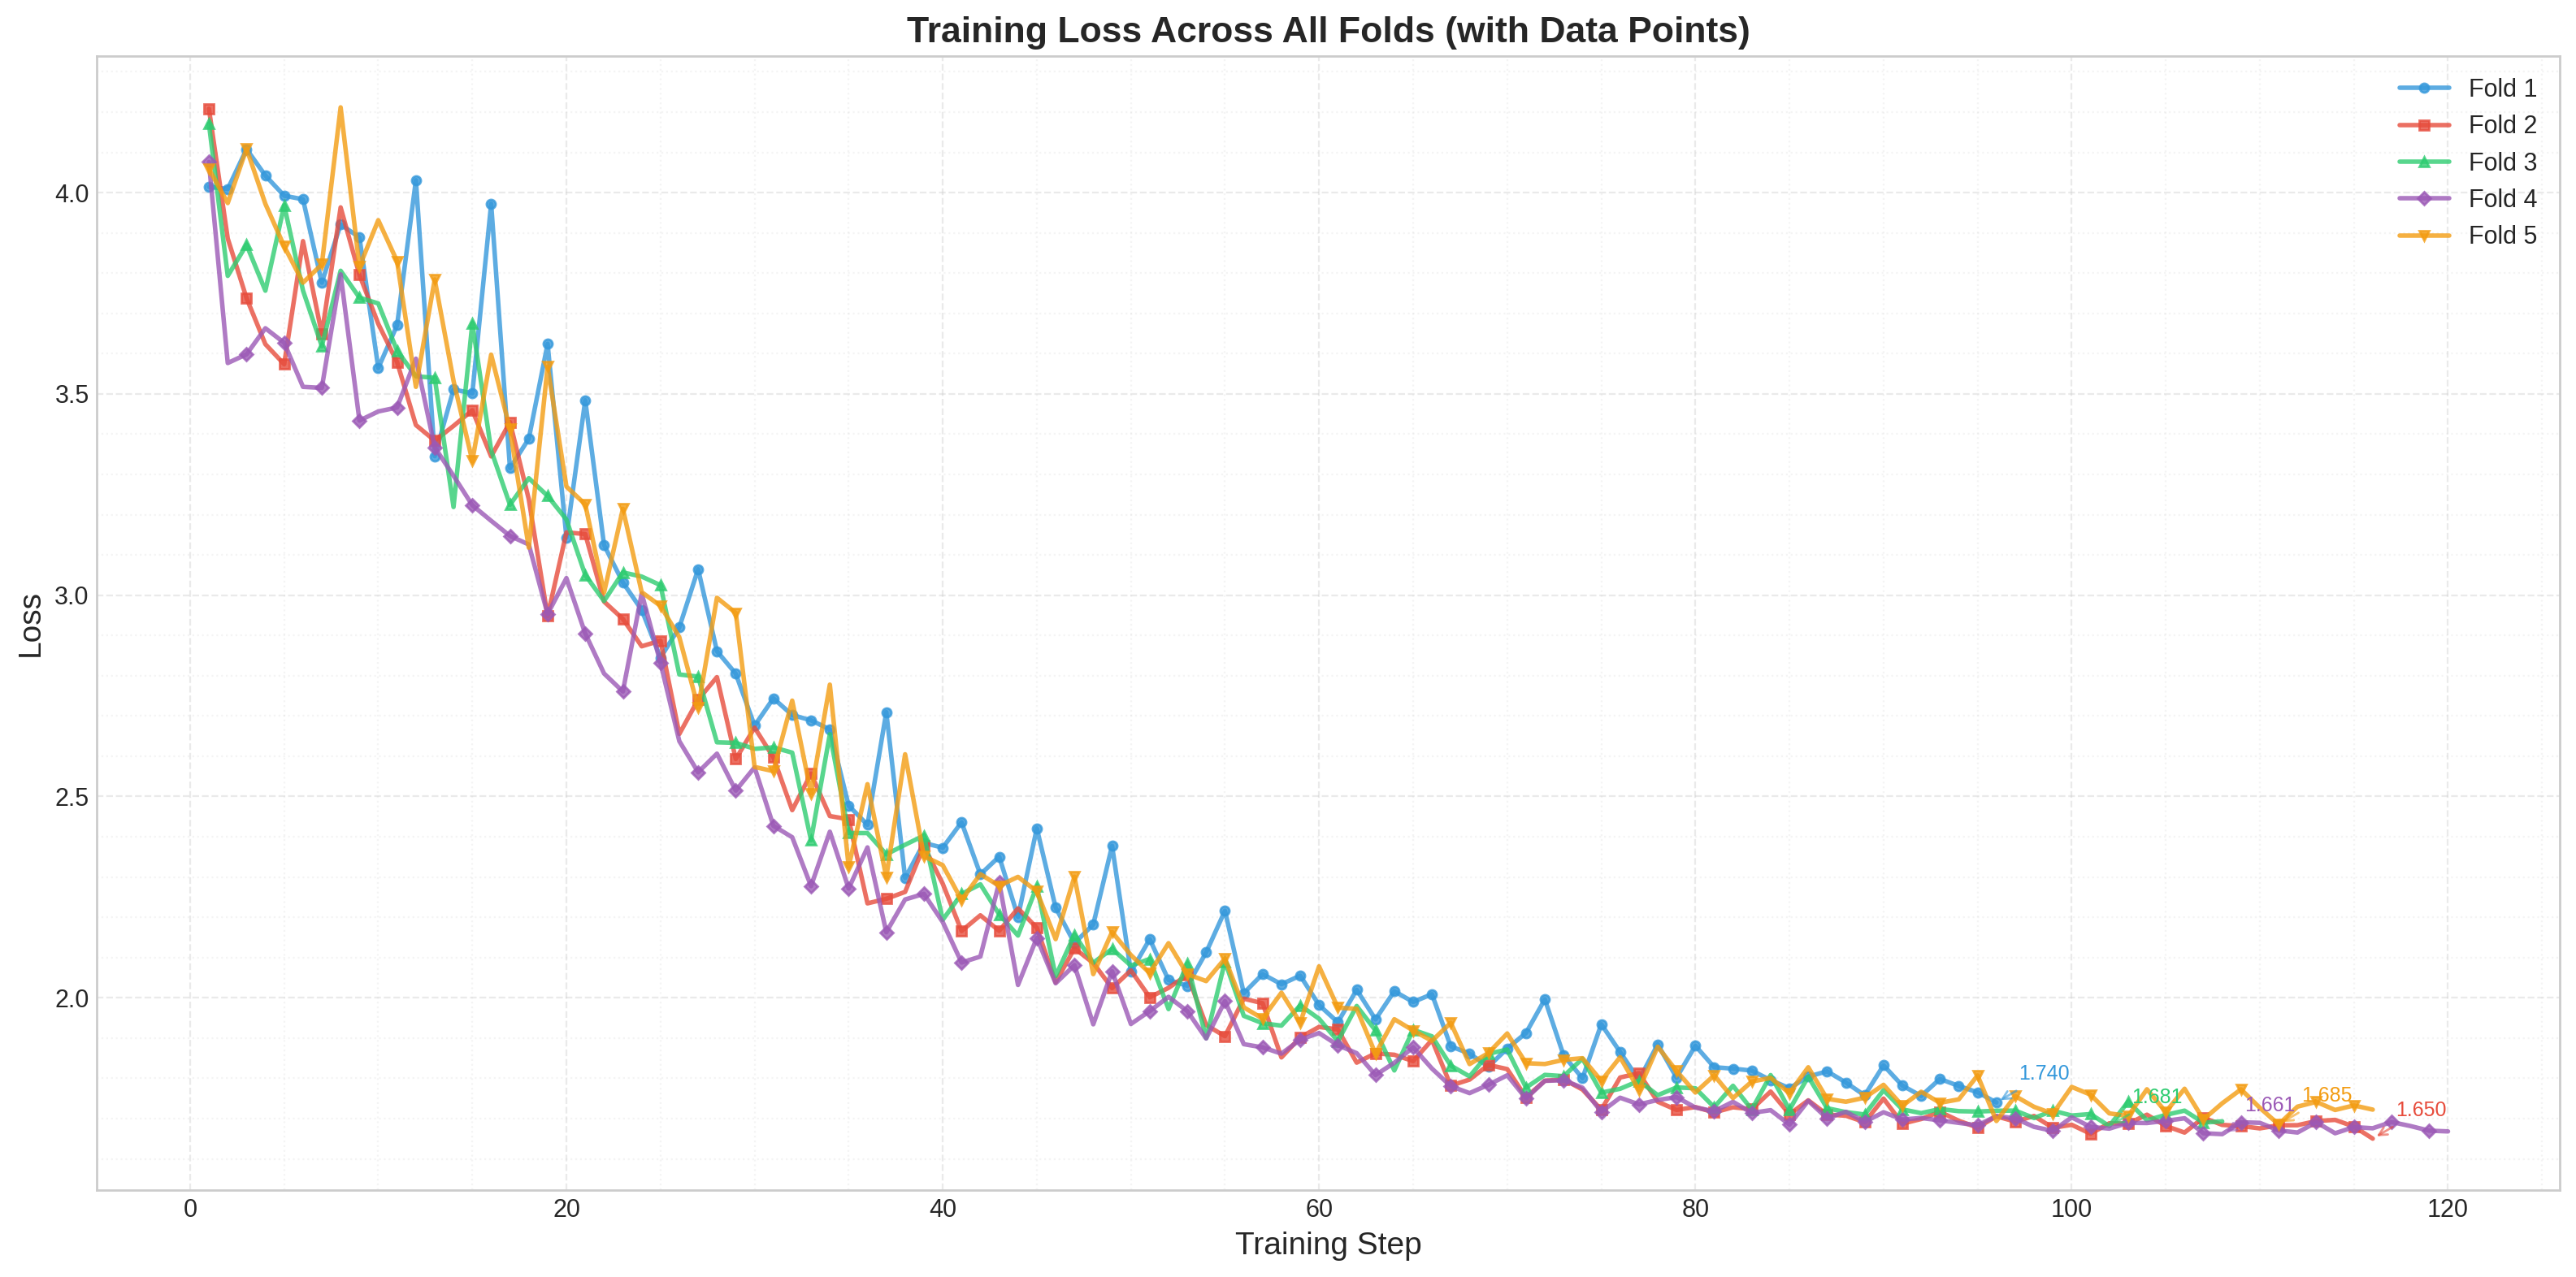
\includegraphics[width=0.8\textwidth]{code/freeze_encoder/outputs/metrics/run_20260212_060037/visualizations/training_loss_detailed.png}
\caption{Kurva Training Loss --- Strategi Freeze Encoder}
\label{fig:fe_training_loss}
\end{figure}

Tabel~\ref{tab:fe_training_summary} merangkum statistik training untuk setiap \textit{fold}:

\begin{table}[H]
\centering
\caption{Ringkasan Training Freeze Encoder per Fold}
\label{tab:fe_training_summary}
\begin{tabular}{|c|c|c|c|c|}
\hline
\textbf{Fold} & \textbf{Steps} & \textbf{Initial Loss} & \textbf{Final Loss} & \textbf{Epoch} \\
\hline
0 & 96 & 4,014 & 1,740 & 24 \\
\hline
1 & 116 & 4,208 & 1,650 & 29 \\
\hline
2 & 108 & 4,171 & 1,693 & 27 \\
\hline
3 & 120 & 4,076 & 1,668 & 30 \\
\hline
4 & 116 & 4,059 & 1,722 & 29 \\
\hline
\hline
\textbf{Mean} & \textbf{111,2} & \textbf{4,106} & \textbf{1,695} & \textbf{27,8} \\
\hline
\end{tabular}
\end{table}

Seluruh \textit{fold} berhasil menurunkan \textit{training loss} dari kisaran 4,0--4,2 menjadi $\sim$1,7. Tidak seperti Run 1--4 sebelumnya yang tanpa \textit{label smoothing} di mana loss menurun hingga $\sim$0,01, Run 5 menggunakan \textit{label smoothing factor} 0,1 yang secara sengaja mendistribusikan probabilitas ke seluruh \textit{vocabulary}, sehingga loss minimum teoritis bukan 0 melainkan $\sim$1,5 \cite{szegedy2016rethinking}. Hal ini mencegah model menjadi terlalu percaya diri (\textit{overconfident}) dan berfungsi sebagai regularisasi tambahan. \textit{Early stopping} (\textit{patience}=6 steps) berhasil menghentikan training sebelum batas 120 steps pada semua \textit{fold}.

\subsection{Metrik Evaluasi Freeze Encoder}

Gambar~\ref{fig:fe_eval_metrics} menunjukkan perkembangan WER dan CER selama evaluasi pada strategi \textit{Freeze Encoder}.

\begin{figure}[H]
\centering
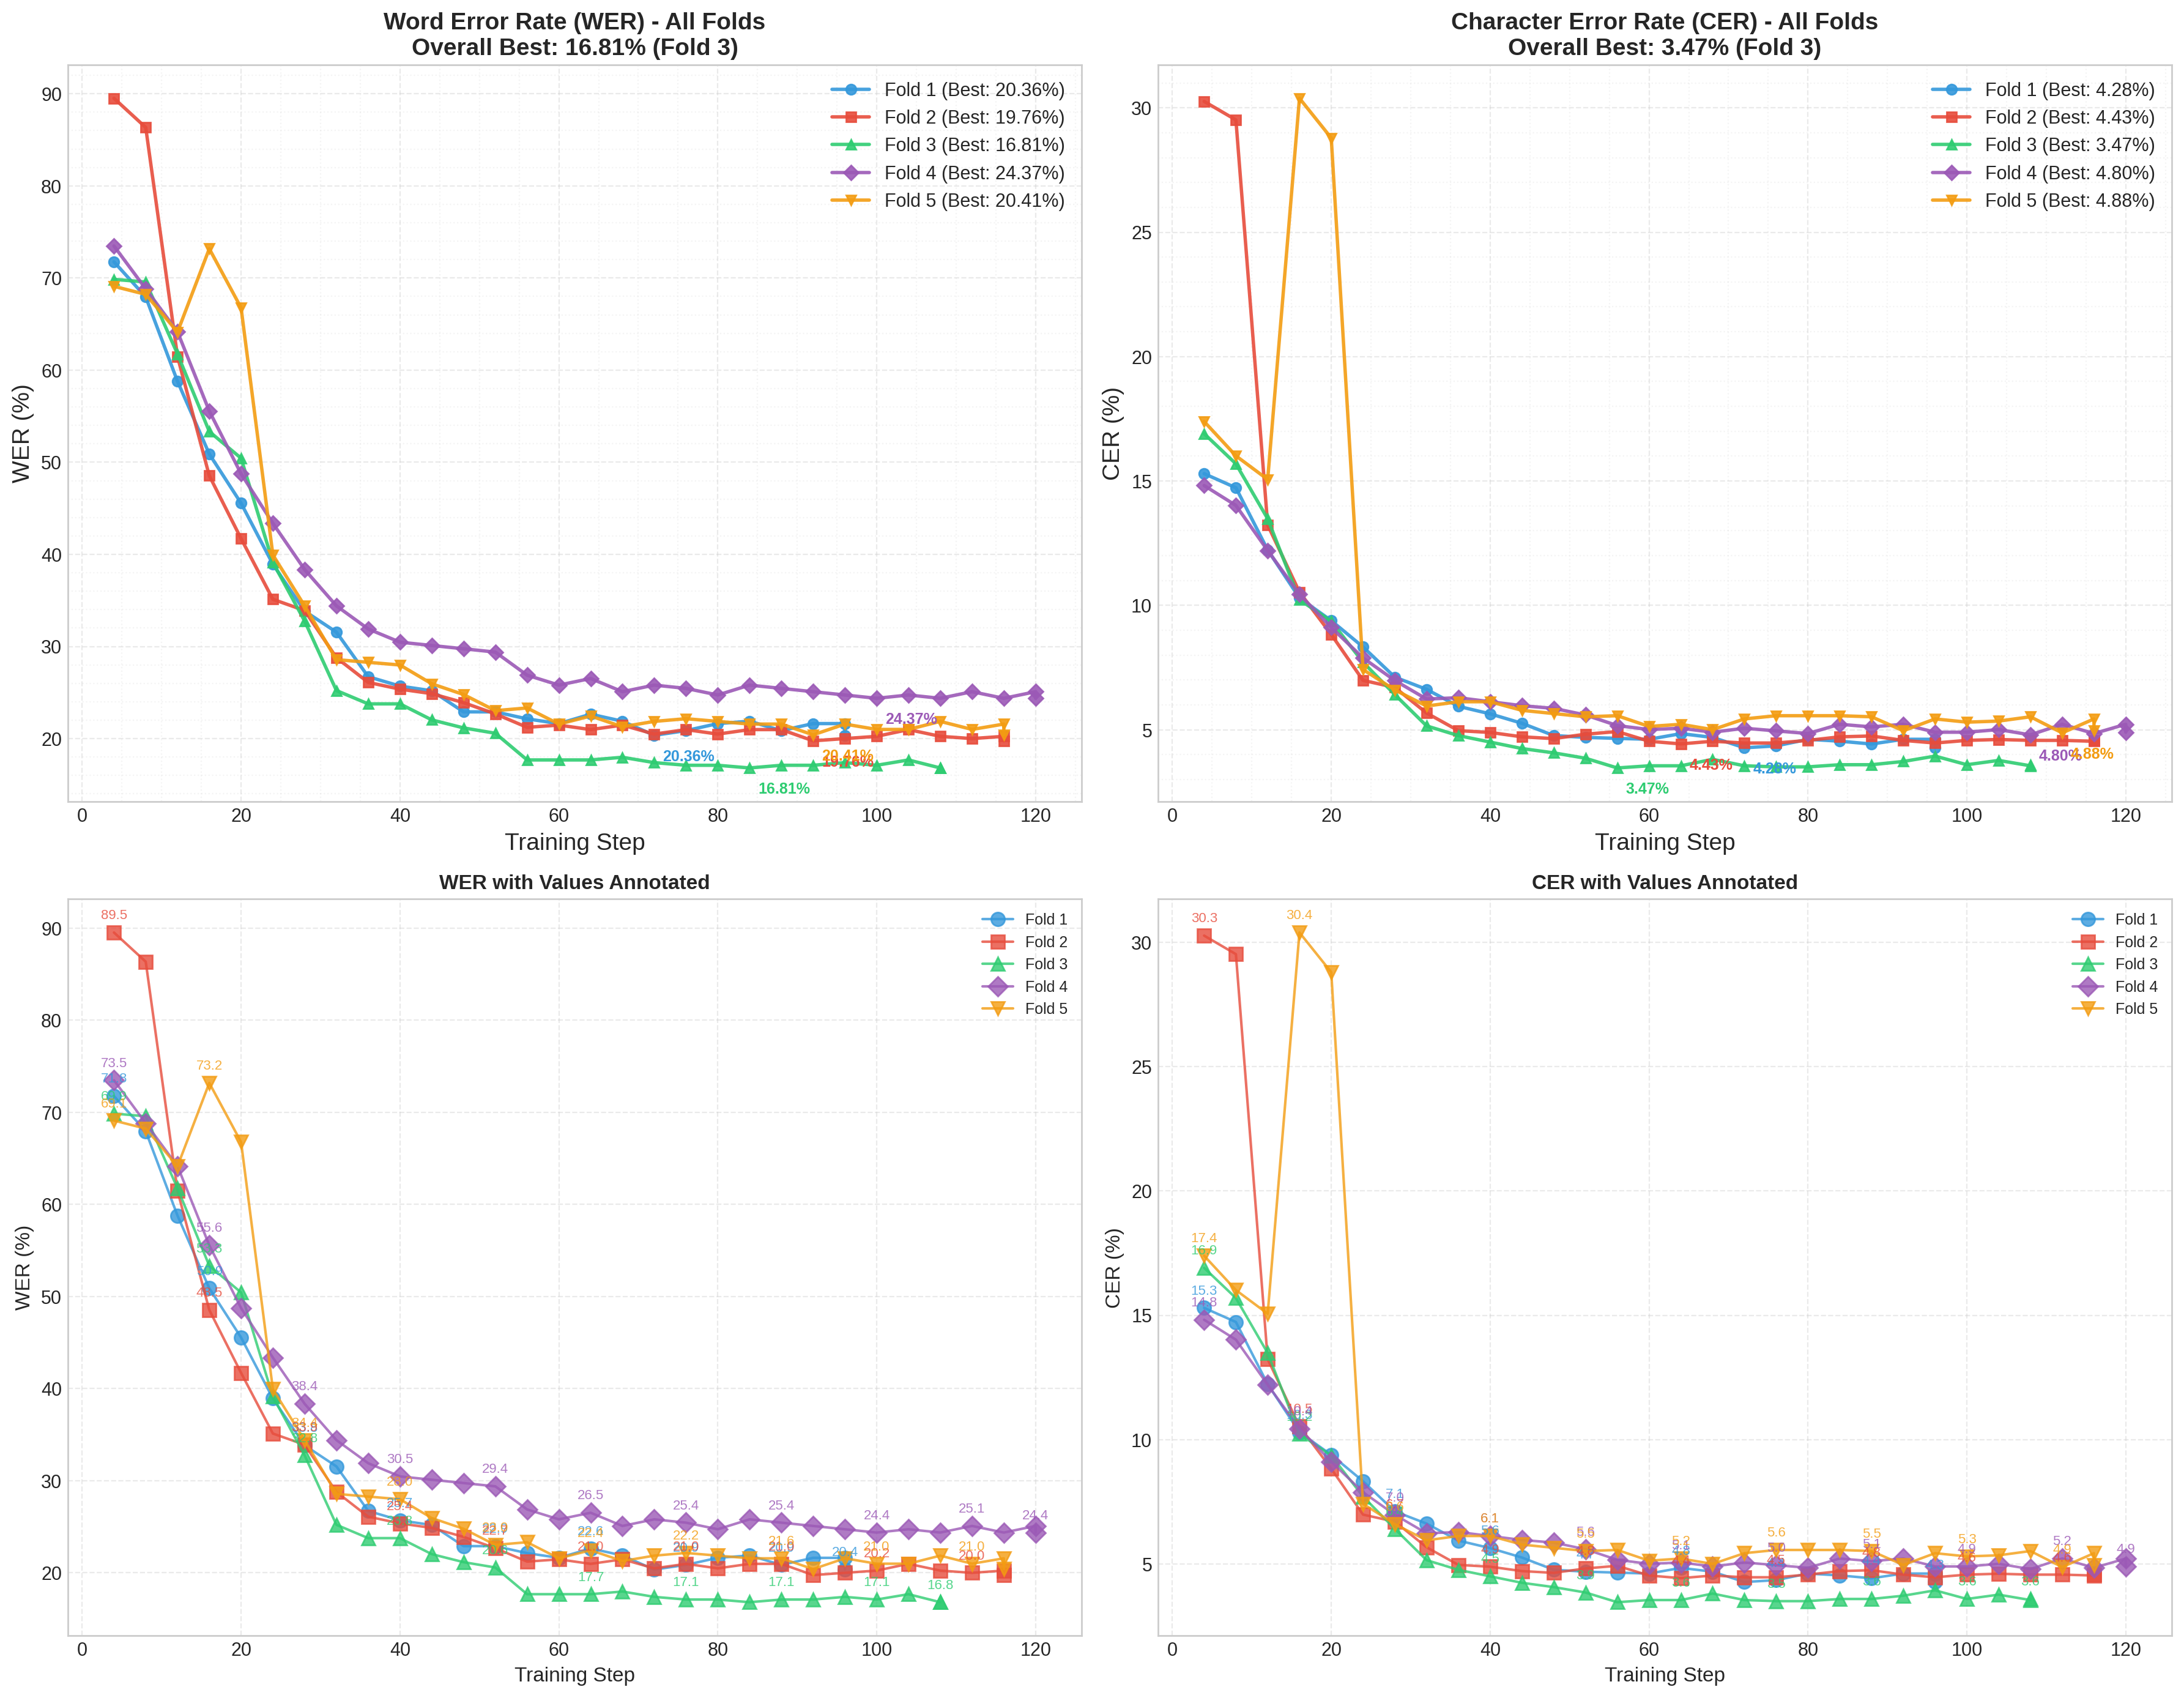
\includegraphics[width=0.9\textwidth]{code/freeze_encoder/outputs/metrics/run_20260212_060037/visualizations/evaluation_metrics_detailed.png}
\caption{Perkembangan WER dan CER --- Strategi Freeze Encoder}
\label{fig:fe_eval_metrics}
\end{figure}

Semua \textit{fold} menunjukkan penurunan WER yang signifikan dari rentang 70--73\% pada evaluasi awal menjadi 16--24\% pada evaluasi akhir. Beberapa pola penting yang teramati:

\begin{itemize}
    \item \textbf{Penurunan WER yang Cepat}: Sebagian besar penurunan WER terjadi pada 40--60 \textit{steps} pertama ($\sim$10--15 \textit{epochs}), di mana WER turun dari $>$70\% menjadi $\sim$25--30\%. Setelah itu, penurunan berlangsung lebih lambat dan bertahap menuju nilai konvergen.
    
    \item \textbf{Variasi Antar-Fold yang Tinggi}: Terdapat perbedaan yang cukup besar antar-\textit{fold} pada fase akhir training. \textit{Fold}~2 mencapai WER terendah (16,81\%) sementara \textit{Fold}~3 hanya mencapai 24,37\%, dengan rentang 7,56 poin persentase. Variasi ini mengindikasikan sensitivitas tinggi terhadap komposisi data training dan evaluasi pada dataset kecil.
    
    \item \textbf{CER Lebih Stabil}: Dibandingkan WER, kurva CER menunjukkan konvergensi yang lebih seragam antar-\textit{fold} dengan rentang akhir yang lebih sempit (3,60\%--4,96\%), menunjukkan bahwa kesalahan karakter lebih konsisten meskipun kesalahan kata bervariasi.
    
    \item \textbf{Fluktuasi pada Beberapa Fold}: Beberapa \textit{fold} menunjukkan fluktuasi metrik evaluasi pada fase pertengahan training, yang mengindikasikan ketidakstabilan optimasi akibat dataset yang sangat kecil dan jumlah parameter trainable yang besar (37M, 50\% dari total).
\end{itemize}

\subsection{Prediksi Model Freeze Encoder}

Tabel~\ref{tab:fe_predictions_fold2} menampilkan contoh prediksi pada \textit{Fold}~2 (fold terbaik, WER 16,81\%):

\begin{table}[H]
\centering
\caption{Contoh Prediksi Freeze Encoder pada Fold 2 (Fold Terbaik)}
\label{tab:fe_predictions_fold2}
\resizebox{\textwidth}{!}{%
\begin{tabular}{|p{0.42\textwidth}|p{0.42\textwidth}|c|c|}
\hline
\textbf{Referensi} & \textbf{Prediksi Model} & \textbf{WER} & \textbf{CER} \\
\hline
manusia sadonyo lahia ka dunia mambao hak hak dan kamardekaan mandasar nan samo dan indak dapek dipisahkan & 
manusia sadonyonyo lahia kadunian mambuh hak hak dan kamardekaan mandasar nan samo dan indak dapek dipisahkan & 
23,5\% & 5,7\% \\
\hline
sasungguahnyo ikrar negara negara anggota & 
susungguahnyo iklar negara negara anggota & 
40,0\% & 6,7\% \\
\hline
untuak mamajukan panghormatan taradok hak hak asasi manusia dan kamardekaan nan mandasar & 
untuak mamajukan pangormatan taradok hak hak asasi manusia dan kamardekaan nan mandasar & 
\textbf{8,3\%} & \textbf{1,1\%} \\
\hline
\end{tabular}%
}
\end{table}

Pola kesalahan utama pada \textit{Freeze Encoder} meliputi: (1) substitusi fonetik pada konsonan serupa (``deklarasi'' $\rightarrow$ ``rekelerasi'', ``sasungguahnyo'' $\rightarrow$ ``susungguahnyo''); (2) kesalahan segmentasi kata (``di antaro'' $\rightarrow$ ``diantaro'', ``anggota alah'' $\rightarrow$ ``anggotaalah''); dan (3) variasi partikel Minangkabau (``mampatahankannyo'' $\rightarrow$ ``mampatahankan jo'').

%% ====================================================================
%% SECTION: HASIL LoRA
%% ====================================================================
\section{Hasil Strategi LoRA} \label{IV.LoRA}

\subsection{Perbandingan Eksperimen LoRA}

Serupa dengan strategi \textit{Freeze Encoder}, dilakukan lima kali percobaan pelatihan (\textit{run}) dengan strategi LoRA untuk menemukan konfigurasi optimal. Setiap percobaan menggunakan variasi \textit{hyperparameter} yang berbeda, termasuk variasi \textit{rank}, \textit{learning rate}, \textit{weight decay}, dan \textit{dropout}. Tabel~\ref{tab:lora_run_configs} merangkum konfigurasi yang digunakan pada setiap percobaan.

\begin{table}[H]
\centering
\caption{Konfigurasi Hyperparameter Lima Percobaan LoRA}
\label{tab:lora_run_configs}
\resizebox{\textwidth}{!}{%
\begin{tabular}{|l|c|c|c|c|c|}
\hline
\textbf{Parameter} & \textbf{Run 1} & \textbf{Run 2} & \textbf{Run 3} & \textbf{Run 4} & \textbf{Run 5} \\
 & \textbf{(8 Feb, 16:30)} & \textbf{(8 Feb, 17:44)} & \textbf{(8 Feb, 18:51)} & \textbf{(8 Feb, 19:41)} & \textbf{(12 Feb, 06:32)} \\
\hline
\hline
\multicolumn{6}{|c|}{\textbf{Konfigurasi LoRA Adapter}} \\
\hline
Rank ($r$) & 8 & 8 & 16 & 8 & 8 \\
\hline
Alpha ($\alpha$) & 16 & 16 & 32 & 16 & 16 \\
\hline
Scaling ($\alpha / r$) & 2,0$\times$ & 2,0$\times$ & 2,0$\times$ & 2,0$\times$ & 2,0$\times$ \\
\hline
LoRA Dropout & 0,1 & 0,1 & 0,15 & 0,15 & 0,15 \\
\hline
Target Modules & \multicolumn{5}{c|}{q\_proj, v\_proj, k\_proj, out\_proj, fc1, fc2} \\
\hline
\hline
\multicolumn{6}{|c|}{\textbf{Konfigurasi Training}} \\
\hline
Learning Rate & 5$\times$10\textsuperscript{-4} & 5$\times$10\textsuperscript{-4} & 3$\times$10\textsuperscript{-4} & 7$\times$10\textsuperscript{-4} & 7$\times$10\textsuperscript{-4} \\
\hline
Batch Size & 32 & 32 & 32 & 32 & 32 \\
\hline
Max Steps & 400 & 400 & 250 & 250 & 200 \\
\hline
Warmup Ratio & 0,1 & 0,1 & 0,15 & 0,1 & 0,1 \\
\hline
Weight Decay & 0,01 & 0,01 & 0,03 & 0,05 & 0,05 \\
\hline
Label Smoothing & 0,1 & 0,1 & 0,05 & 0,1 & 0,1 \\
\hline
\hline
\multicolumn{6}{|c|}{\textbf{Konfigurasi Dropout Model}} \\
\hline
Decoder Dropout & 0,1 & 0,1 & 0,15 & 0,1 & 0,1 \\
\hline
Attention Dropout & 0,05 & 0,05 & 0,1 & 0,05 & 0,05 \\
\hline
Activation Dropout & 0,05 & 0,05 & 0,1 & 0,05 & 0,05 \\
\hline
\hline
\multicolumn{6}{|c|}{\textbf{Decoding}} \\
\hline
Beam Width & 5 & 5 & 5 & 5 & 5 \\
\hline
\end{tabular}%
}
\end{table}

Tabel~\ref{tab:lora_run_comparison} merangkum hasil performa dari seluruh percobaan LoRA.

\begin{table}[H]
\centering
\caption{Perbandingan Hasil Lima Percobaan LoRA}
\label{tab:lora_run_comparison}
\resizebox{\textwidth}{!}{%
\begin{tabular}{|c|c|c|c|c|c|c|c|}
\hline
\textbf{Run} & \textbf{Rank} & \textbf{LR} & \textbf{Weight Decay} & \textbf{Label Smooth.} & \textbf{Mean WER (\%)} & \textbf{Mean CER (\%)} & \textbf{Std WER (\%)} \\
\hline
\textbf{1 (16:30)} & \textbf{8} & \textbf{5$\times$10\textsuperscript{-4}} & \textbf{0,01} & \textbf{0,1} & \textbf{17,32 $\pm$ 0,83} & \textbf{3,49 $\pm$ 0,43} & \textbf{0,83} \\
\hline
2 (17:44) & 8 & 5$\times$10\textsuperscript{-4} & 0,01 & 0,1 & 17,73 $\pm$ 1,91 & 3,57 $\pm$ 0,33 & 1,91 \\
\hline
3 (18:51) & 16 & 3$\times$10\textsuperscript{-4} & 0,03 & 0,05 & 18,03 $\pm$ 1,01 & 3,80 $\pm$ 0,39 & 1,01 \\
\hline
4 (19:41) & 8 & 7$\times$10\textsuperscript{-4} & 0,05 & 0,1 & 17,43 $\pm$ 1,74 & 3,78 $\pm$ 0,53 & 1,74 \\
\hline
5 (12 Feb) & 8 & 7$\times$10\textsuperscript{-4} & 0,05 & 0,1 & 17,87 $\pm$ 2,06 & 3,51 $\pm$ 0,53 & 2,06 \\
\hline
\end{tabular}%
}
\end{table}

Run 1 tetap mencapai WER rata-rata terbaik (\textbf{17,32\%}) dan konsistensi tertinggi (std WER 0,83\%), namun Run 5 dipilih sebagai konfigurasi akhir karena menggunakan \textit{learning rate} yang lebih tinggi (7$\times$10\textsuperscript{-4}) dan \textit{weight decay} yang lebih kuat (0,05) sehingga konfigurasi regularisasinya lebih seimbang. Run 5 mencapai WER 17,87\% dengan CER yang kompetitif (3,51\%). Beberapa temuan dari eksplorasi \textit{hyperparameter} LoRA:

\begin{enumerate}
    \item \textbf{Run 1 vs Run 2} (konfigurasi identik): Run 2 merupakan pengulangan Run 1 dengan konfigurasi yang sama, menghasilkan WER rata-rata yang sangat mirip (17,73\% vs 17,32\%), namun dengan standar deviasi yang lebih tinggi (1,91\% vs 0,83\%). Perbedaan ini menunjukkan variabilitas inheren dari \textit{stochastic training} dan inisialisasi \textit{adapter} LoRA yang acak.
    
    \item \textbf{Run 3} (rank lebih tinggi, LR lebih rendah): Peningkatan \textit{rank} dari 8 ke 16 (menggandakan parameter trainable) dengan \textit{learning rate} yang lebih rendah (3$\times$10\textsuperscript{-4}) dan \textit{label smoothing} yang lebih kecil (0,05) justru menghasilkan WER yang lebih tinggi (18,03\%). Hal ini mengindikasikan bahwa pada dataset sekecil ini, peningkatan kapasitas model tidak selalu bermanfaat---\textit{rank} 8 sudah cukup untuk mengkodekan adaptasi yang diperlukan.
    
    \item \textbf{Run 4 vs Run 5} (reproduktibilitas \textit{v3 config}): Kedua run menggunakan konfigurasi yang identik (LR=7$\times$10\textsuperscript{-4}, WD=0,05, LS=0,1, LoRA dropout=0,15), namun menghasilkan WER yang berbeda (17,43\% vs 17,87\%) dengan standar deviasi yang juga berbeda (1,74\% vs 2,06\%). Variasi ini konsisten dengan temuan Run 1 vs Run 2, mengkonfirmasi bahwa variabilitas $\sim$0,5 poin persentase WER merupakan \textit{noise} inheren dari \textit{stochastic training}.
\end{enumerate}

Analisis selanjutnya menggunakan hasil dari \textbf{Run 5} (lora\_20260212\_063207) karena menggunakan konfigurasi akhir yang telah dioptimasi berdasarkan temuan Run 1--4.

\subsection{Konfigurasi LoRA Terbaik}

Tabel~\ref{tab:lora_config} merangkum konfigurasi LoRA pada Run 1 yang digunakan untuk analisis mendalam.

\begin{table}[H]
\centering
\caption{Konfigurasi LoRA Terbaik (Run 1)}
\label{tab:lora_config}
\begin{tabular}{|l|l|}
\hline
\textbf{Parameter} & \textbf{Nilai} \\
\hline
Rank ($r$) & 8 \\
\hline
Alpha ($\alpha$) & 16 \\
\hline
Scaling ($\alpha / r$) & 2,0$\times$ \\
\hline
LoRA Dropout & 0,1 \\
\hline
Target Modules & q\_proj, v\_proj, k\_proj, out\_proj, fc1, fc2 \\
\hline
Modules to Save & --- (kosong) \\
\hline
Bias & none \\
\hline
\hline
\textbf{Total Parameter} & \textbf{73.675.264} \\
\hline
\textbf{Parameter Trainable} & \textbf{1.081.344 (1,47\%)} \\
\hline
\textbf{Parameter Frozen} & \textbf{72.593.920 (98,53\%)} \\
\hline
\end{tabular}
\end{table}

Dengan konfigurasi ini, hanya \textbf{1,47\%} parameter yang dilatih---jauh lebih efisien dibandingkan \textit{Freeze Encoder} (50\%) maupun \textit{full fine-tuning} (100\%). LoRA menargetkan semua enam \textit{linear layer} pada setiap blok \textit{attention} dan \textit{feed-forward}: \texttt{q\_proj}, \texttt{v\_proj}, \texttt{k\_proj}, \texttt{out\_proj}, \texttt{fc1}, dan \texttt{fc2} \cite{hu2022lora}. Konfigurasi training menggunakan \textit{learning rate} 5$\times$10\textsuperscript{-4} (50$\times$ lebih tinggi dari \textit{Freeze Encoder}), \textit{weight decay} 0,01, \textit{label smoothing} 0,1, dan skema \textit{dropout} yang lebih ringan (\textit{dropout}=0,1; \textit{attention dropout}=0,05; \textit{activation dropout}=0,05) karena jumlah parameter trainable yang jauh lebih kecil mengurangi risiko \textit{overfitting} secara inheren.

\subsection{Hasil Cross-Validation LoRA}

Tabel~\ref{tab:lora_cv_results} menunjukkan hasil evaluasi 5-\textit{fold cross-validation} untuk strategi LoRA.

\begin{table}[H]
\centering
\caption{Hasil 5-Fold Cross-Validation Strategi LoRA}
\label{tab:lora_cv_results}
\begin{tabular}{|c|c|c|c|c|c|}
\hline
\textbf{Fold} & \textbf{Train} & \textbf{Eval} & \textbf{WER (\%)} & \textbf{CER (\%)} & \textbf{Steps} \\
\hline
0 & 124 & 32 & 16,79 & 3,22 & 72 \\
\hline
1 & 125 & 31 & 17,32 & 3,48 & 68 \\
\hline
2 & 125 & 31 & \textbf{15,36} & \textbf{2,86} & 136 \\
\hline
3 & 125 & 31 & 21,51 & 3,57 & 76 \\
\hline
4 & 125 & 31 & 18,37 & 4,45 & 76 \\
\hline
\hline
\textbf{Mean} & \textbf{125} & \textbf{31} & \textbf{17,87 $\pm$ 2,06} & \textbf{3,51 $\pm$ 0,53} & \textbf{85,6} \\
\hline
\end{tabular}
\end{table}

Strategi LoRA mencapai rata-rata WER \textbf{17,87\% $\pm$ 2,06\%} dan CER \textbf{3,51\% $\pm$ 0,53\%}. Beberapa observasi penting:

\begin{itemize}
    \item \textbf{Variasi antar-Fold}: Rentang WER antar-\textit{fold} mencapai 6,15 poin persentase (15,36\%--21,51\%), yang menunjukkan bahwa komposisi data pada tiap \textit{fold} cukup mempengaruhi performa model. Standar deviasi WER (2,06\%) sebanding dengan \textit{Freeze Encoder} (2,41\%), mengindikasikan bahwa variabilitas ini lebih disebabkan oleh karakteristik dataset daripada metode pelatihan.
    
    \item \textbf{Fold Terbaik}: \textit{Fold}~2 mencapai WER terendah (15,36\%) sekaligus CER terendah (2,86\%). Konsistensi antara WER dan CER terbaik pada \textit{fold} yang sama menunjukkan bahwa \textit{Fold}~2 memiliki distribusi data evaluasi yang paling sesuai dengan pola yang dipelajari model.
    
    \item \textbf{Fold Terburuk}: \textit{Fold}~3 menunjukkan WER tertinggi (21,51\%) dengan CER 3,57\%. Kesenjangan besar antara \textit{Fold}~3 dan \textit{fold} lainnya ($>$3 poin persentase WER) mengindikasikan adanya sampel-sampel sulit yang terkonsentrasi pada \textit{fold} ini.
    
    \item \textbf{Efisiensi \textit{Steps}}: Rata-rata \textit{steps} hanya 85,6 (dari maks 200), jauh lebih rendah dibanding Run 1 (136,0 \textit{steps} dari maks 400). \textit{Early stopping} yang lebih cepat menunjukkan bahwa model dengan konfigurasi \textit{weight decay} 0,05 konvergen lebih cepat.
\end{itemize}

\subsection{Konvergensi Training LoRA}

Gambar~\ref{fig:lora_training_loss} menampilkan kurva \textit{training loss} untuk strategi LoRA.

\begin{figure}[H]
\centering
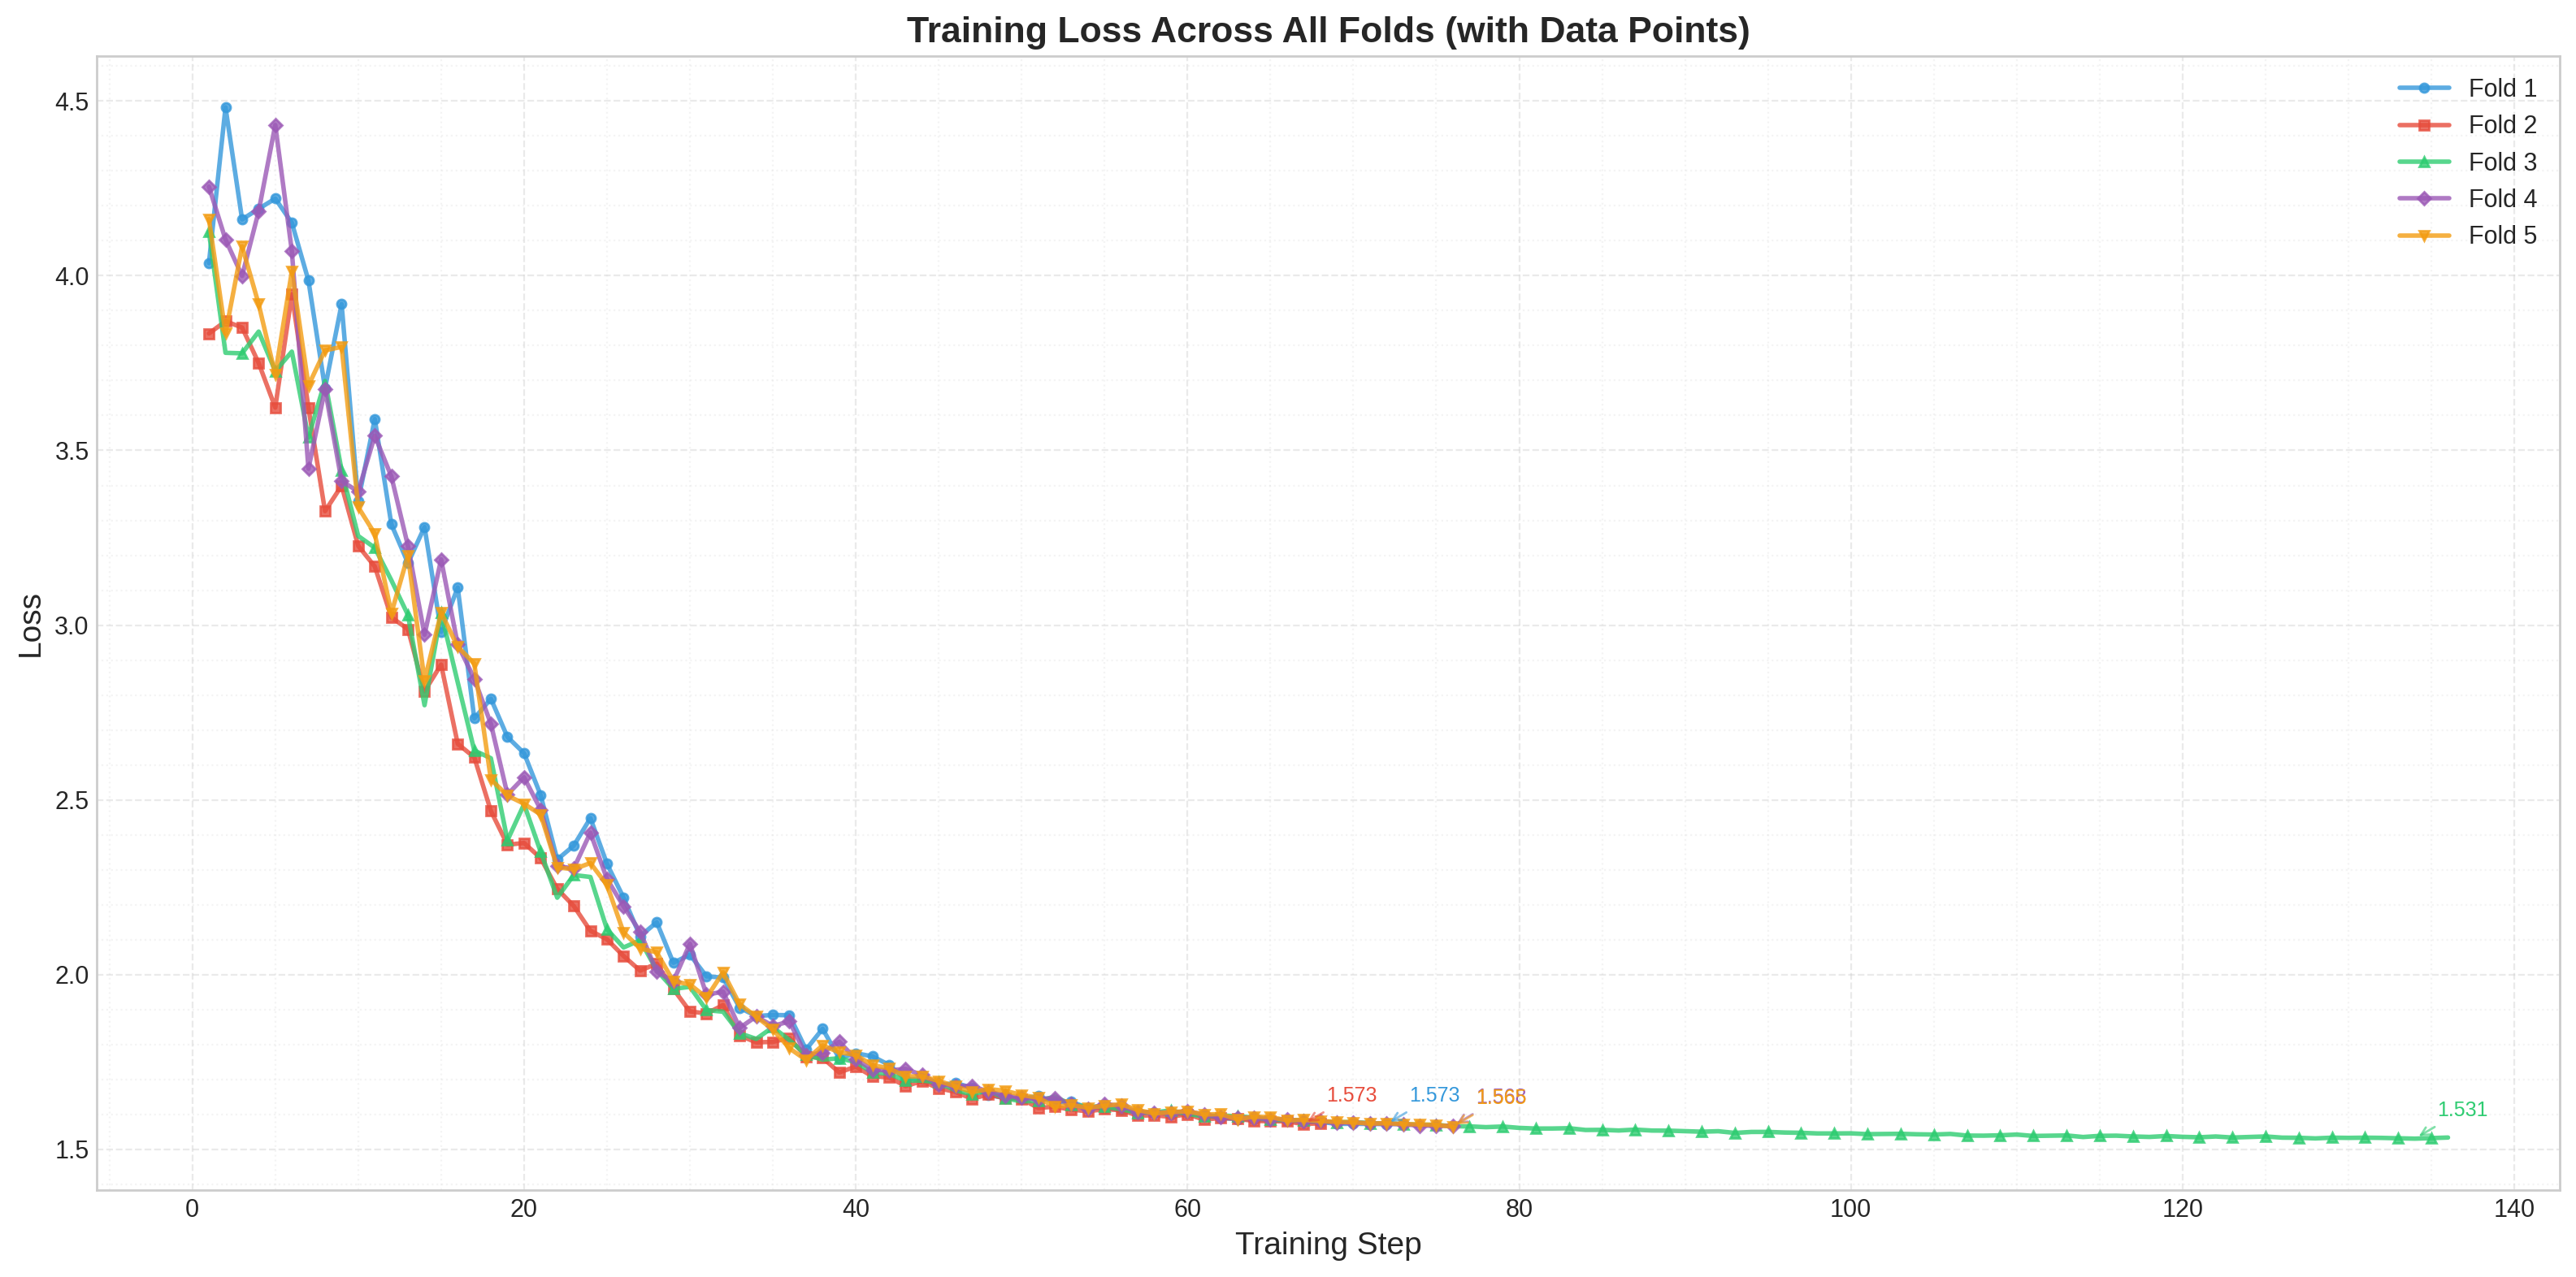
\includegraphics[width=0.8\textwidth]{code/lora/outputs/metrics/lora_20260212_063207/visualizations/training_loss_detailed.png}
\caption{Kurva Training Loss --- Strategi LoRA}
\label{fig:lora_training_loss}
\end{figure}

Tabel~\ref{tab:lora_training_summary} merangkum statistik training LoRA:

\begin{table}[H]
\centering
\caption{Ringkasan Training LoRA per Fold}
\label{tab:lora_training_summary}
\begin{tabular}{|c|c|c|c|c|}
\hline
\textbf{Fold} & \textbf{Steps} & \textbf{Initial Loss} & \textbf{Final Loss} & \textbf{Epoch} \\
\hline
0 & 72 & 4,036 & 1,573 & 18 \\
\hline
1 & 68 & 3,835 & 1,575 & 17 \\
\hline
2 & 136 & 4,126 & 1,534 & 34 \\
\hline
3 & 76 & 4,255 & 1,568 & 19 \\
\hline
4 & 76 & 4,162 & 1,565 & 19 \\
\hline
\hline
\textbf{Mean} & \textbf{85,6} & \textbf{4,083} & \textbf{1,563} & \textbf{21,4} \\
\hline
\end{tabular}
\end{table}

Pola konvergensi LoRA menunjukkan karakteristik yang berbeda dari \textit{Freeze Encoder}:

\begin{itemize}
    \item \textbf{Initial Loss yang Konsisten}: LoRA memulai dengan loss rata-rata 4,08 (rentang 3,84--4,26), mirip dengan \textit{Freeze Encoder} yang juga menggunakan \textit{label smoothing} (4,00--4,20). Kesamaan \textit{initial loss} ini diharapkan karena kedua strategi menggunakan \textit{label smoothing factor} yang sama (0,1) yang mendominasi nilai loss awal.
    
    \item \textbf{Final Loss Konvergen}: Loss akhir LoRA ($\sim$1,56) konvergen ke nilai yang serupa dengan \textit{Freeze Encoder} ($\sim$1,70), keduanya di sekitar batas minimum teoritis yang ditentukan oleh \textit{label smoothing}. Loss LoRA sedikit lebih rendah karena jumlah parameter trainable yang lebih kecil (1,47\% vs 50\%) memberikan regularisasi implisit tambahan \cite{szegedy2016rethinking}.
    
    \item \textbf{Konvergensi Cepat dengan \textit{Early Stopping}}: Rata-rata hanya memerlukan 85,6 \textit{steps} (21,4 epoch), jauh lebih sedikit dibanding \textit{Freeze Encoder} (111,2 \textit{steps}, 27,8 epoch). Namun \textit{Fold}~2 memerlukan 136 \textit{steps} (34 epoch), hampir dua kali lipat rata-rata \textit{fold} lainnya, menunjukkan bahwa fold ini memiliki distribusi data yang memerlukan waktu adaptasi lebih lama---dan justru menghasilkan performa terbaik.
    
    \item \textbf{Efisiensi Parameter}: Meskipun hanya melatih 1,47\% parameter (vs 50\%), LoRA mencapai WER rata-rata yang lebih baik (17,87\% vs 20,34\%). Hal ini menunjukkan bahwa \textit{low-rank adaptation} mampu mengekstraksi kapasitas pembelajaran yang cukup dari modifikasi parameter yang sangat terbatas.
\end{itemize}

\subsection{Metrik Evaluasi LoRA}

Gambar~\ref{fig:lora_eval_metrics} menunjukkan perkembangan WER dan CER selama evaluasi.

\begin{figure}[H]
\centering
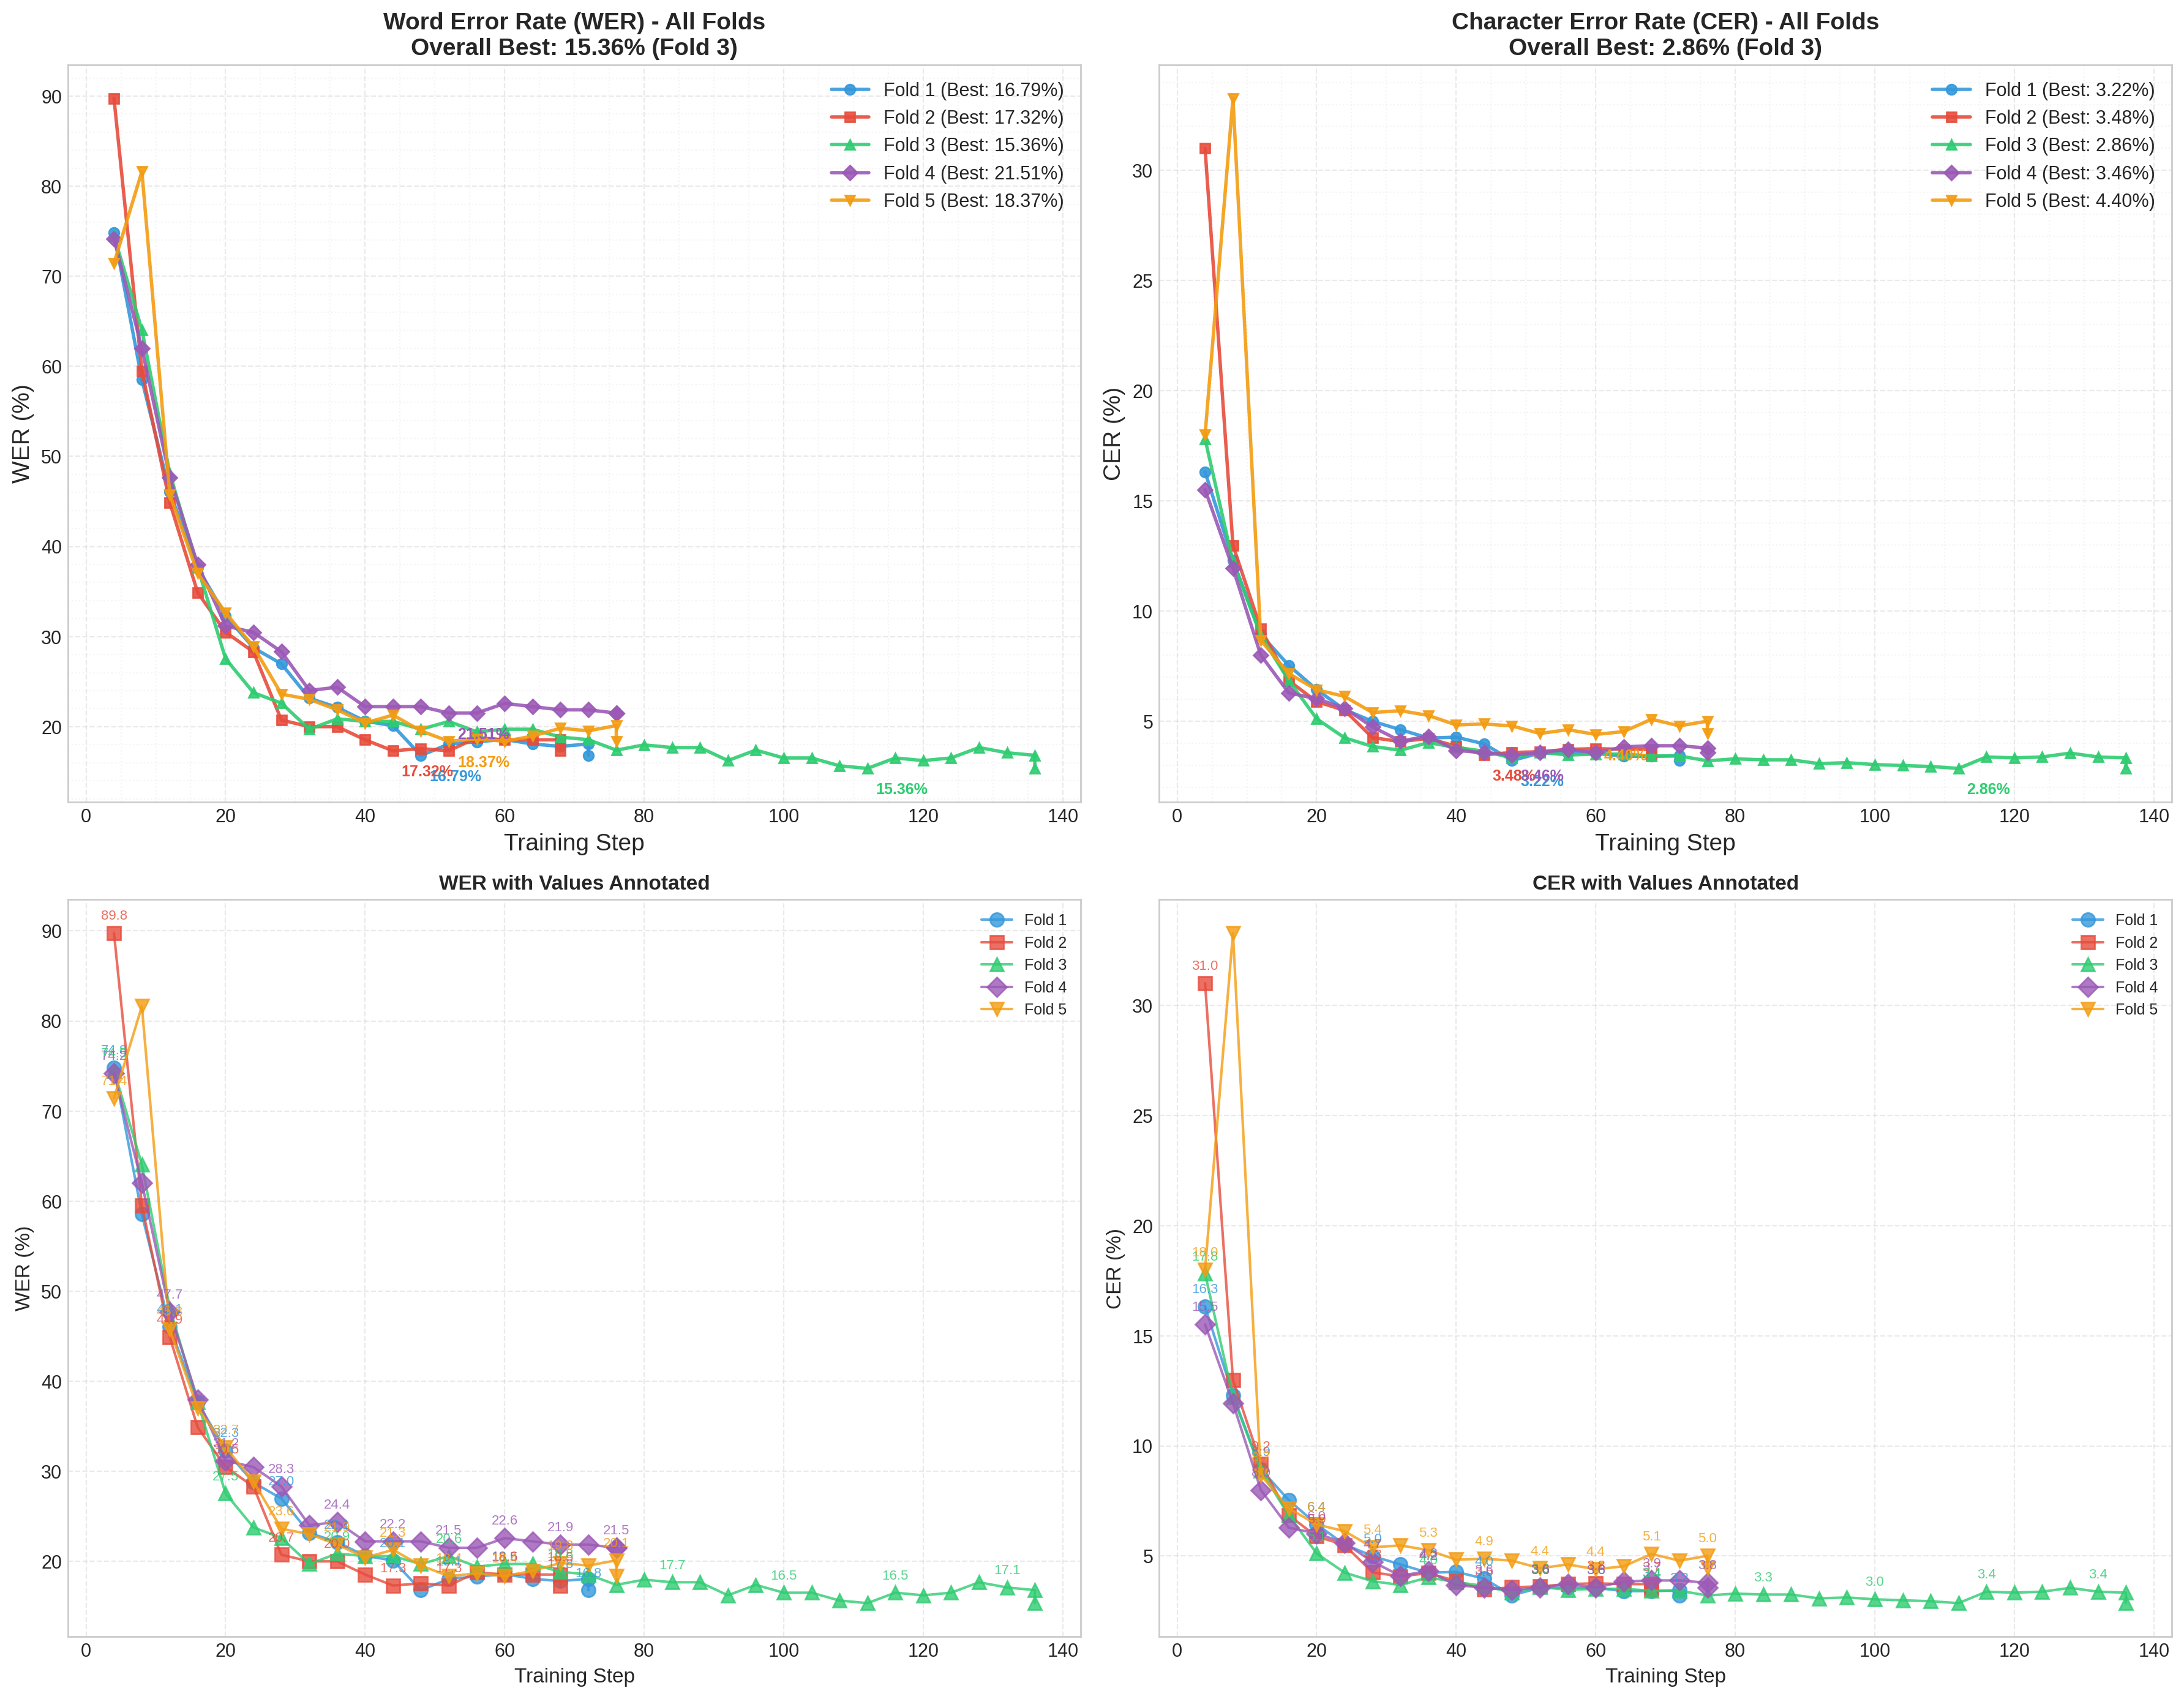
\includegraphics[width=0.9\textwidth]{code/lora/outputs/metrics/lora_20260212_063207/visualizations/evaluation_metrics_detailed.png}
\caption{Perkembangan WER dan CER --- Strategi LoRA}
\label{fig:lora_eval_metrics}
\end{figure}

Semua \textit{fold} menunjukkan penurunan WER dari rentang tinggi pada evaluasi awal menjadi 15--22\% pada evaluasi akhir. \textit{Fold}~2 yang memerlukan \textit{steps} terbanyak (136) menunjukkan kurva konvergensi yang lebih gradual, sementara \textit{fold} lainnya (68--76 \textit{steps}) konvergen lebih cepat. Konvergensi metrik evaluasi menunjukkan stabilitas yang baik tanpa fluktuasi berlebihan, konsisten dengan efek regularisasi dari \textit{label smoothing} dan jumlah parameter trainable yang sangat terbatas.

\subsection{Prediksi Model LoRA}

Tabel~\ref{tab:lora_predictions_fold2} menampilkan contoh prediksi pada \textit{Fold}~2 (fold terbaik WER, 15,36\%):

\begin{table}[H]
\centering
\caption{Contoh Prediksi LoRA pada Fold 2 (Fold Terbaik WER)}
\label{tab:lora_predictions_fold2}
\resizebox{\textwidth}{!}{%
\begin{tabular}{|p{0.42\textwidth}|p{0.42\textwidth}|c|c|}
\hline
\textbf{Referensi} & \textbf{Prediksi Model} & \textbf{WER} & \textbf{CER} \\
\hline
dalam deklarasi sadunia hak hak asasi manusia & 
dalam deklarasi sadunia hak hak asasi manusia & 
\textbf{0,0\%} & \textbf{0,0\%} \\
\hline
untuak mamajukan panghormatan taradok hak hak asasi manusia dan kamardekaan nan mandasar & 
untuak mamajukan panghormatan taradok hak hak asasi manusia dan kamardekaan nan mandasar & 
\textbf{0,0\%} & \textbf{0,0\%} \\
\hline
punyo hak mandapek linduangan masyarakat jo negara & 
punyo hak mandapek linduangan masyarakat jo negara & 
\textbf{0,0\%} & \textbf{0,0\%} \\
\hline
hak ko indak balaku untuak dakwaan kajahatan non politik & 
hak ko indak balaku untuak daquan kajahatan non politik & 
11,1\% & 5,4\% \\
\hline
\end{tabular}%
}
\end{table}

Sebagai perbandingan, Tabel~\ref{tab:lora_predictions_fold3} menampilkan contoh prediksi dari \textit{Fold}~3 (fold terburuk WER, 21,51\%):

\begin{table}[H]
\centering
\caption{Contoh Prediksi LoRA pada Fold 3 (Fold Terburuk WER)}
\label{tab:lora_predictions_fold3}
\resizebox{\textwidth}{!}{%
\begin{tabular}{|p{0.42\textwidth}|p{0.42\textwidth}|c|c|}
\hline
\textbf{Referensi} & \textbf{Prediksi Model} & \textbf{WER} & \textbf{CER} \\
\hline
hak hak ko adolah milik awak & 
hak hak ko adolah milik awak & 
\textbf{0,0\%} & \textbf{0,0\%} \\
\hline
hak hak asasi manusia paralu dijamin malalui tartib hukum & 
hak hak asasi manusia paralu dijamin malalui tartib hukum & 
\textbf{0,0\%} & \textbf{0,0\%} \\
\hline
kalompok atau sasaurang & 
kalompok atau saso urang & 
66,7\% & 8,7\% \\
\hline
baitu pulo kahormatan jo namo baiaknyo & 
baitu pulo kah rumah tan jo nan mo baiknyo & 
100,0\% & 18,4\% \\
\hline
\end{tabular}%
}
\end{table}

Pola kesalahan LoRA menunjukkan karakteristik yang khas:

\begin{enumerate}
    \item \textbf{Prediksi Sempurna}: Pada \textit{Fold}~2, 9 dari 31 sampel (29\%) diprediksi sempurna, sementara pada \textit{Fold}~3 hanya 5 dari 31 (16\%). Kalimat pendek cenderung diprediksi dengan benar.
    
    \item \textbf{Segmentasi Kata}: Kesalahan ``dakwaan'' $\rightarrow$ ``daquan'' dan ``sasaurang'' $\rightarrow$ ``saso urang'' menunjukkan tantangan dalam mengenali batas kata dan \textit{compound word} dalam bahasa Minangkabau. Kata ``sasaurang'' yang seharusnya satu kata dipecah menjadi dua kata oleh model.
    
    \item \textbf{Hallusinasi pada Kalimat Pendek}: Pada \textit{Fold}~3, prediksi ``kahormatan jo namo baiaknyo'' $\rightarrow$ ``kah rumah tan jo nan mo baiknyo'' (WER 100\%) menunjukkan \textit{hallucination} yang signifikan dimana model menghasilkan kata-kata yang secara fonetik mirip tetapi secara semantik berbeda. Ini merupakan tantangan khas pada dataset kecil.
    
    \item \textbf{CER Tetap Terkontrol}: Bahkan pada prediksi dengan WER tertinggi (100\%), CER tetap moderat (18,4\%), mengkonfirmasi bahwa kesalahan lebih bersifat \textit{word-level} daripada \textit{character-level}.
\end{enumerate}

%% ====================================================================
%% SECTION: PERBANDINGAN STRATEGI
%% ====================================================================
\section{Perbandingan Strategi Fine-Tuning} \label{IV.Perbandingan}

\subsection{Ringkasan Seluruh Percobaan}

Tabel~\ref{tab:all_runs_summary} menyajikan ringkasan hasil dari seluruh sepuluh percobaan (lima \textit{Freeze Encoder} dan lima LoRA) yang dilakukan selama penelitian.

\begin{table}[H]
\centering
\caption{Ringkasan Seluruh Percobaan Training}
\label{tab:all_runs_summary}
\resizebox{\textwidth}{!}{%
\begin{tabular}{|c|l|c|c|c|c|c|c|}
\hline
\textbf{No.} & \textbf{Strategi} & \textbf{LR} & \textbf{Batch} & \textbf{W. Decay} & \textbf{Beam} & \textbf{Mean WER (\%)} & \textbf{Mean CER (\%)} \\
\hline
\hline
\multicolumn{8}{|c|}{\textbf{Freeze Encoder}} \\
\hline
FE-1 & Freeze Encoder & 5$\times$10\textsuperscript{-6} & 16$\times$2 & 0,2 & 1 & 25,07 $\pm$ 2,86 & 5,60 $\pm$ 0,59 \\
\hline
FE-2 & Freeze Encoder & 1$\times$10\textsuperscript{-5} & 16$\times$2 & 0,2 & 1 & 22,34 $\pm$ 1,89 & 4,93 $\pm$ 0,55 \\
\hline
FE-3 & Freeze Encoder & 1$\times$10\textsuperscript{-5} & 16$\times$2 & 0,2 & 1 & 22,95 $\pm$ 2,70 & 5,52 $\pm$ 0,77 \\
\hline
FE-4 & Freeze Encoder & 1$\times$10\textsuperscript{-5} & 32$\times$1 & 0,1 & 5 & 19,92 $\pm$ 2,42 & 4,53 $\pm$ 0,65 \\
\hline
\textbf{FE-5} & \textbf{Freeze Encoder} & \textbf{1$\times$10\textsuperscript{-5}} & \textbf{32$\times$1} & \textbf{0,1} & \textbf{5} & \textbf{20,34 $\pm$ 2,41} & \textbf{4,46 $\pm$ 0,50} \\
\hline
\hline
\multicolumn{8}{|c|}{\textbf{LoRA}} \\
\hline
L-1 & LoRA ($r$=8) & 5$\times$10\textsuperscript{-4} & 32 & 0,01 & 5 & 17,32 $\pm$ 0,83 & 3,49 $\pm$ 0,43 \\
\hline
L-2 & LoRA ($r$=8) & 5$\times$10\textsuperscript{-4} & 32 & 0,01 & 5 & 17,73 $\pm$ 1,91 & 3,57 $\pm$ 0,33 \\
\hline
L-3 & LoRA ($r$=16) & 3$\times$10\textsuperscript{-4} & 32 & 0,03 & 5 & 18,03 $\pm$ 1,01 & 3,80 $\pm$ 0,39 \\
\hline
L-4 & LoRA ($r$=8) & 7$\times$10\textsuperscript{-4} & 32 & 0,05 & 5 & 17,43 $\pm$ 1,74 & 3,78 $\pm$ 0,53 \\
\hline
\textbf{L-5} & \textbf{LoRA ($r$=8)} & \textbf{7$\times$10\textsuperscript{-4}} & \textbf{32} & \textbf{0,05} & \textbf{5} & \textbf{17,87 $\pm$ 2,06} & \textbf{3,51 $\pm$ 0,53} \\
\hline
\end{tabular}%
}
\end{table}

Dari Tabel~\ref{tab:all_runs_summary}, terlihat jelas bahwa \textbf{seluruh percobaan LoRA} (WER 17,32\%--18,03\%) mengungguli \textbf{seluruh percobaan Freeze Encoder} (WER 19,92\%--25,07\%) dalam hal rata-rata WER. Bahkan percobaan LoRA terburuk (L-3, WER 18,03\%) masih lebih baik 1,89 poin persentase dari percobaan \textit{Freeze Encoder} terbaik (FE-4, WER 19,92\%). Hal ini menunjukkan keunggulan yang konsisten dan \textit{robust} dari strategi LoRA pada skenario \textit{low-resource} ini. Run terakhir pada masing-masing strategi (FE-5 dan L-5) dipilih sebagai konfigurasi final karena menggunakan \textit{label smoothing} dan konfigurasi regularisasi yang telah dioptimasi berdasarkan temuan Run 1--4.

\subsection{Perbandingan Metrik Utama}

Tabel~\ref{tab:strategy_comparison} menyajikan perbandingan komprehensif antara kedua strategi \textit{fine-tuning}.

\begin{table}[H]
\centering
\caption{Perbandingan Strategi Freeze Encoder vs LoRA}
\label{tab:strategy_comparison}
\resizebox{\textwidth}{!}{%
\begin{tabular}{|l|c|c|c|}
\hline
\textbf{Metrik} & \textbf{Freeze Encoder} & \textbf{LoRA} & \textbf{Selisih} \\
\hline
\hline
\multicolumn{4}{|c|}{\textbf{Performa}} \\
\hline
Mean WER (\%) & 20,34 $\pm$ 2,41 & \textbf{17,87 $\pm$ 2,06} & $\downarrow$ 2,47 pp \\
\hline
Mean CER (\%) & 4,46 $\pm$ 0,50 & \textbf{3,51 $\pm$ 0,53} & $\downarrow$ 0,95 pp \\
\hline
Best Fold WER (\%) & 16,81 & \textbf{15,36} & $\downarrow$ 1,45 pp \\
\hline
Worst Fold WER (\%) & 24,37 & \textbf{21,51} & $\downarrow$ 2,86 pp \\
\hline
Rentang WER (\%) & 7,56 & \textbf{6,15} & $\downarrow$ 1,41 pp \\
\hline
Std WER (\%) & 2,41 & \textbf{2,06} & $\downarrow$ 0,35 pp \\
\hline
\hline
\multicolumn{4}{|c|}{\textbf{Efisiensi}} \\
\hline
Parameter Trainable & $\sim$37M (50,0\%) & \textbf{$\sim$1,1M (1,47\%)} & 34$\times$ lebih efisien \\
\hline
Rata-rata Steps & 111,2 & \textbf{85,6} & $\downarrow$ 25,6 \\
\hline
Rata-rata Epoch & 27,8 & \textbf{21,4} & $\downarrow$ 6,4 \\
\hline
Learning Rate & 1$\times$10\textsuperscript{-5} & 7$\times$10\textsuperscript{-4} & 70$\times$ lebih tinggi \\
\hline
Weight Decay & 0,1 & 0,05 & 2$\times$ lebih ringan \\
\hline
Label Smoothing & 0,1 & 0,1 & Sama \\
\hline
Dropout (dec/attn/act) & 0,2 / 0,15 / 0,15 & 0,1 / 0,05 / 0,05 & Lebih ringan \\
\hline
\end{tabular}%
}
\end{table}

\subsection{Analisis Perbandingan}

Dari Tabel~\ref{tab:strategy_comparison}, dapat diidentifikasi beberapa temuan kunci:

\begin{enumerate}
    \item \textbf{LoRA Mengungguli Freeze Encoder pada Metrik Rata-Rata}: LoRA mencapai WER \cite{morris2004wer} 17,87\% dibandingkan 20,34\% pada \textit{Freeze Encoder} (penurunan relatif 12,1\%). Penurunan CER juga signifikan: 3,51\% vs 4,46\% (penurunan relatif 21,3\%). Keunggulan ini dicapai dengan hanya melatih 1,47\% parameter---34 kali lebih sedikit dari \textit{Freeze Encoder}.
    
    \item \textbf{LoRA Lebih Konsisten}: Standar deviasi WER LoRA (2,06\%) lebih rendah dibandingkan \textit{Freeze Encoder} (2,41\%), dan rentang WER antar-\textit{fold} LoRA (6,15 pp) juga lebih sempit dibanding \textit{Freeze Encoder} (7,56 pp). Meskipun perbedaan konsistensi tidak sedramatis pada konfigurasi sebelumnya, LoRA tetap menunjukkan stabilitas yang lebih baik.
    
    \item \textbf{LoRA Unggul pada Semua Fold}: Berbeda dengan perbandingan sebelumnya, LoRA kini juga mencapai \textit{best-case fold} yang lebih baik (15,36\% vs 16,81\%). Baik \textit{best-case} maupun \textit{worst-case} LoRA lebih baik dari \textit{Freeze Encoder}, mengkonfirmasi keunggulan yang konsisten di seluruh pembagian data.
    
    \item \textbf{Konvergensi Lebih Cepat}: LoRA rata-rata memerlukan 85,6 \textit{steps} (21,4 epoch) dibandingkan \textit{Freeze Encoder} yang memerlukan 111,2 \textit{steps} (27,8 epoch). Konvergensi yang lebih cepat ini konsisten dengan \textit{learning rate} yang lebih tinggi (70$\times$) dan jumlah parameter trainable yang lebih kecil.
    
    \item \textbf{Strategi Regularisasi Berbeda}: Kedua strategi kini menggunakan \textit{label smoothing} yang sama (0,1), namun \textit{Freeze Encoder} masih memerlukan \textit{dropout} dan \textit{weight decay} yang lebih tinggi karena 50\% parameter yang dilatih berisiko \textit{overfitting} pada dataset kecil. LoRA menggunakan regularisasi yang lebih ringan karena \textit{low-rank constraint} ($r$=8) sendiri sudah berfungsi sebagai regularisasi struktural yang membatasi kapasitas model secara inheren \cite{hu2022lora}.
\end{enumerate}

Gambar~\ref{fig:comparison_cv} mengilustrasikan perbandingan visual performa kedua strategi.

\begin{figure}[H]
\centering
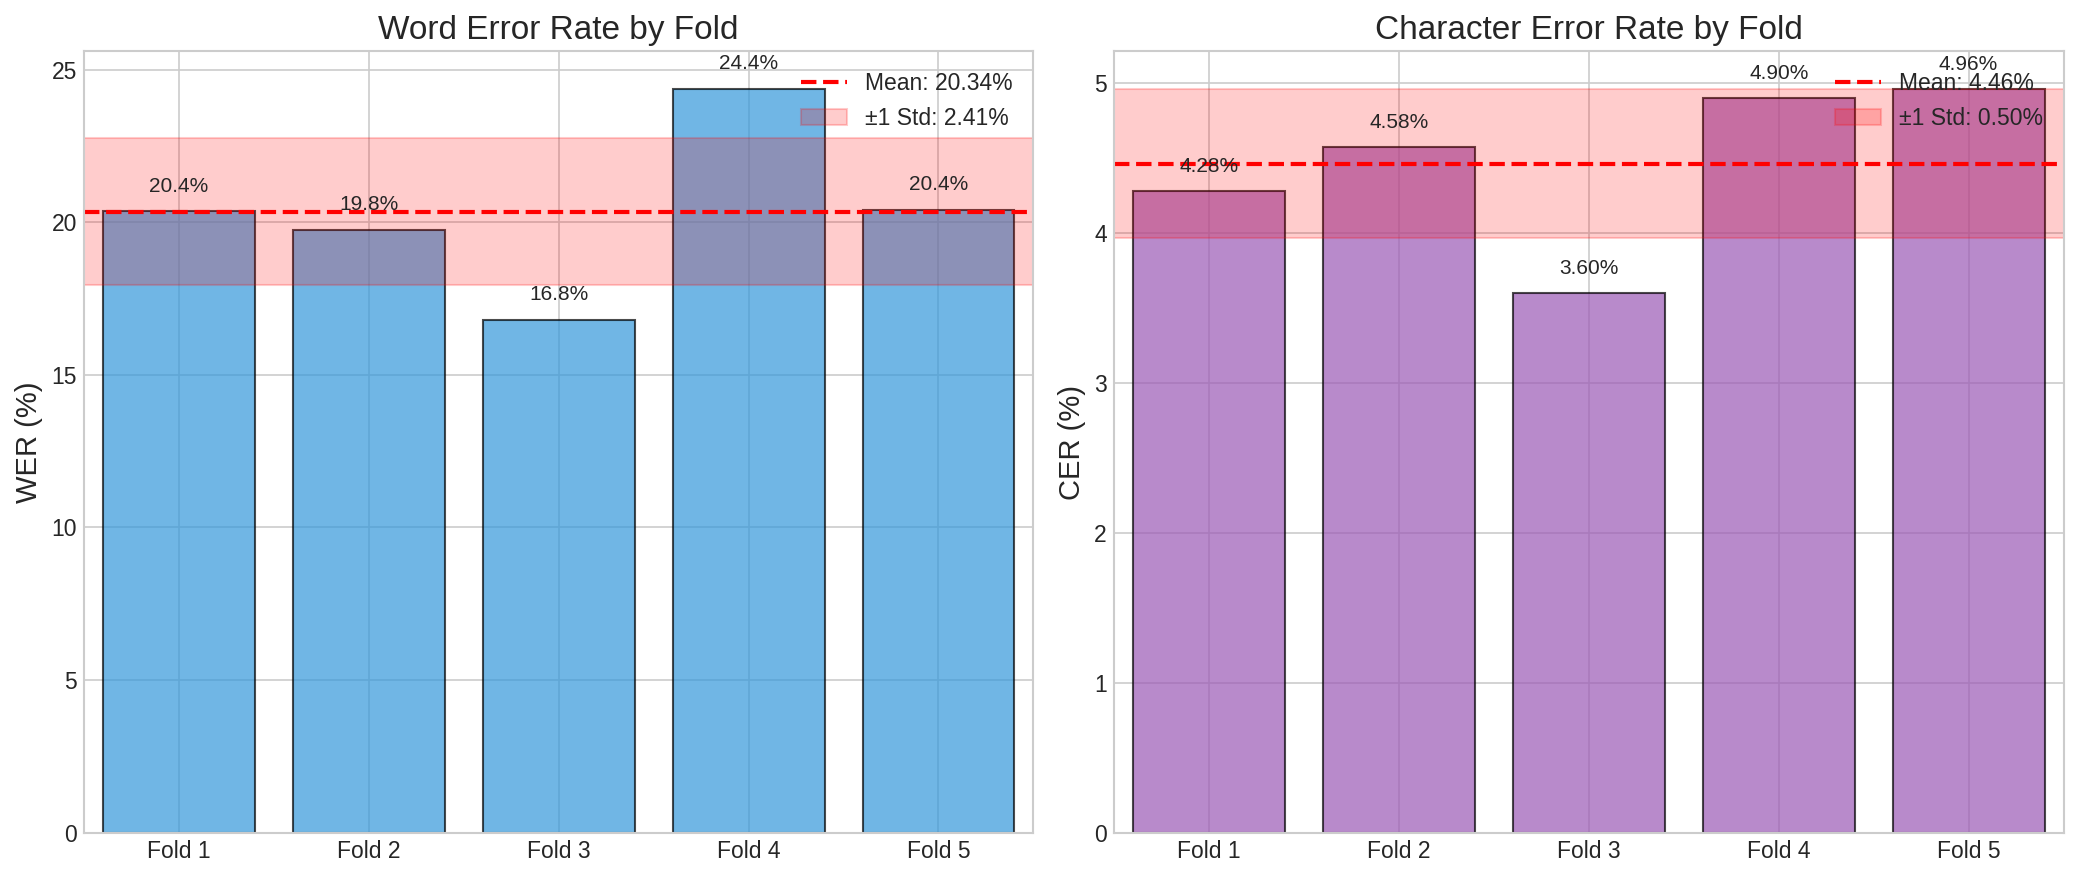
\includegraphics[width=0.9\textwidth]{code/freeze_encoder/outputs/metrics/run_20260212_060037/visualizations/cross_validation_summary.png}
\caption{Cross-Validation Summary --- Freeze Encoder}
\label{fig:comparison_cv}
\end{figure}

\begin{figure}[H]
\centering
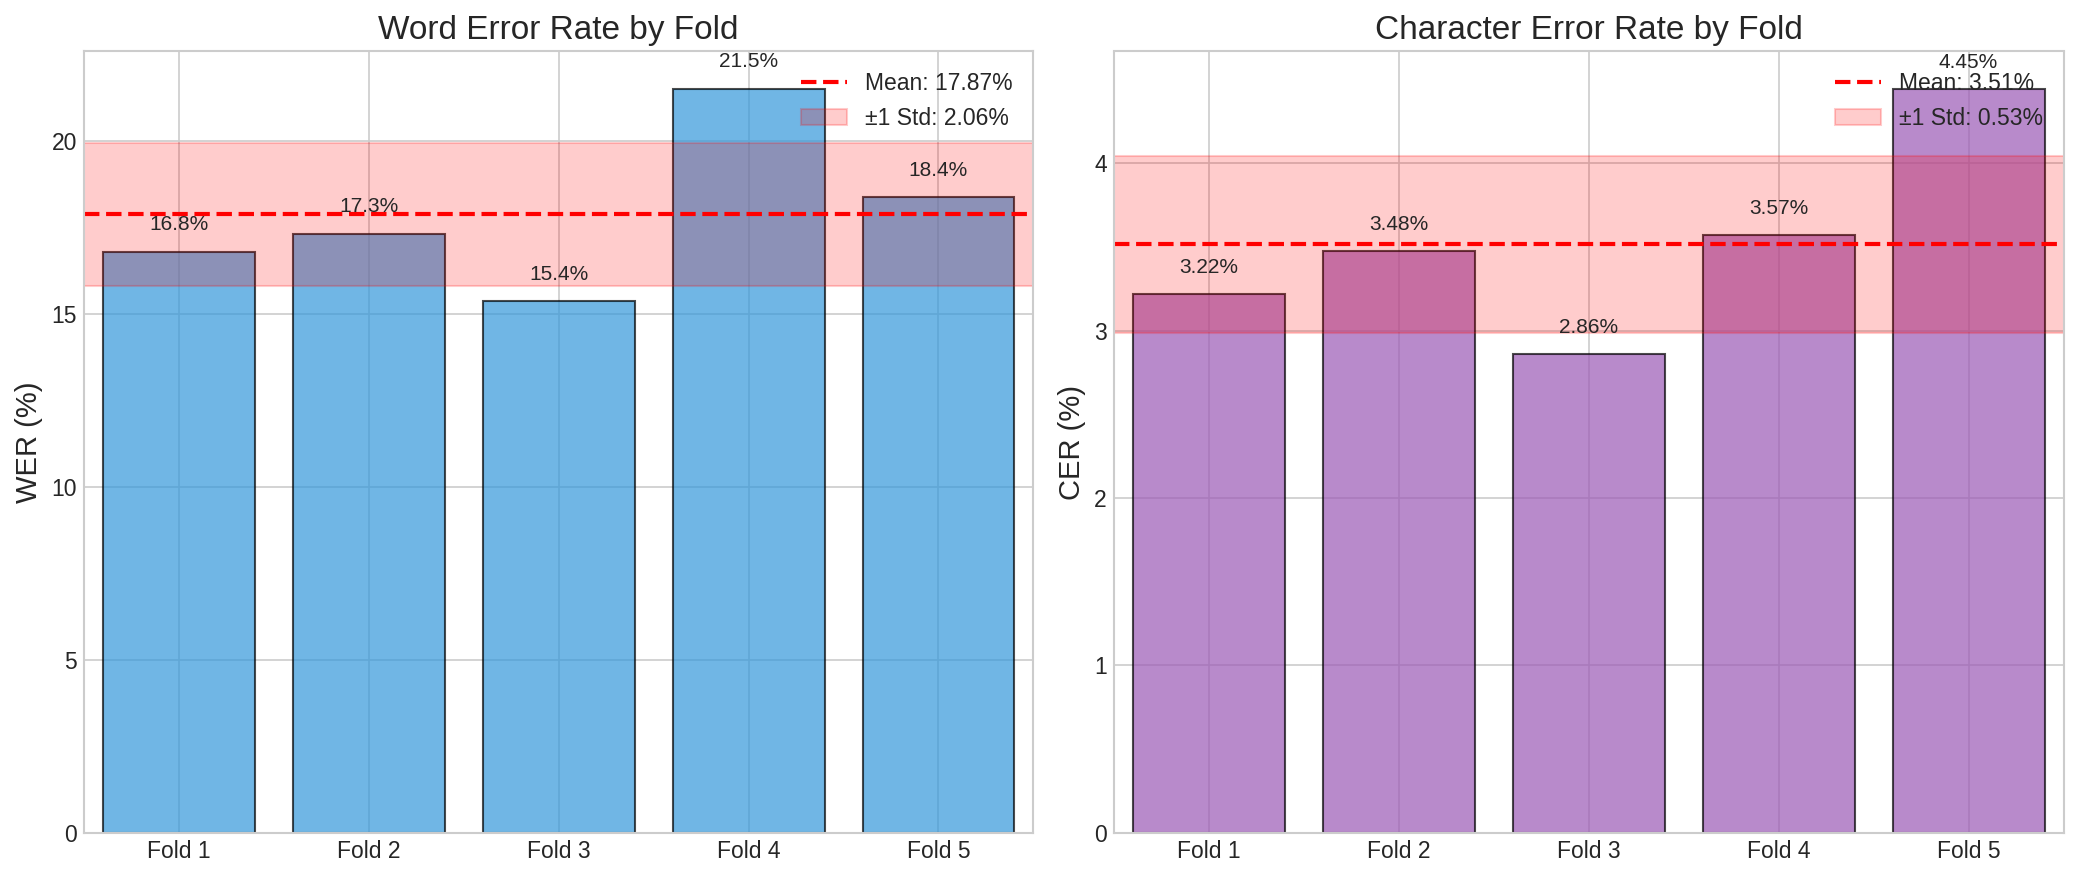
\includegraphics[width=0.9\textwidth]{code/lora/outputs/metrics/lora_20260212_063207/visualizations/cross_validation_summary.png}
\caption{Cross-Validation Summary --- LoRA}
\label{fig:lora_cv_summary}
\end{figure}

%% ====================================================================
%% SECTION: PEMBAHASAN
%% ====================================================================
\section{Pembahasan} \label{IV.Analisis}

\subsection{Efektivitas LoRA pada Skenario Low-Resource}

Keunggulan LoRA atas \textit{Freeze Encoder} pada skenario \textit{extremely low-resource} (1,3 jam) merupakan temuan yang signifikan dan sedikit bertentangan dengan intuisi awal. Secara konvensional, lebih banyak parameter trainable (50\% pada \textit{Freeze Encoder}) seharusnya memberikan kapasitas belajar yang lebih besar. Namun, hasil dari seluruh sepuluh percobaan (lima \textit{Freeze Encoder} dan lima LoRA, lihat Tabel~\ref{tab:all_runs_summary}) secara konsisten menunjukkan sebaliknya---LoRA dengan hanya 1,47\% parameter trainable justru lebih baik pada setiap konfigurasi yang diuji. Beberapa penjelasan untuk fenomena ini:

\begin{itemize}
    \item \textbf{Regularisasi Struktural}: \textit{Low-rank constraint} ($r$=8) membatasi perubahan representasi internal ke subspace berdimensi rendah, secara efektif mencegah \textit{overfitting} tanpa memerlukan regularisasi eksplisit yang agresif. Hal ini krusial pada dataset kecil di mana \textit{overfitting} merupakan risiko utama \cite{hu2022lora}.
    
    \item \textbf{Adaptasi di Seluruh Layer}: LoRA memodifikasi semua 6 \textit{linear layer} di setiap blok transformer (encoder dan decoder), memberikan adaptasi yang terdistribusi merata. Sebaliknya, \textit{Freeze Encoder} hanya memodifikasi decoder, sehingga representasi encoder tetap statis. Meskipun encoder Whisper sudah baik untuk audio umum, adaptasi ringan melalui LoRA pada encoder dapat meningkatkan representasi fitur spesifik untuk karakteristik akustik bahasa Minangkabau.
    
    \item \textbf{Learning Rate Optimal}: LoRA menggunakan learning rate 70$\times$ lebih tinggi (7$\times$10\textsuperscript{-4} vs 1$\times$10\textsuperscript{-5}), yang dimungkinkan oleh jumlah parameter trainable yang sangat kecil. Learning rate yang lebih tinggi memungkinkan adaptasi yang lebih cepat dan eksplorasi ruang parameter yang lebih efektif.
    
    \item \textbf{Label Smoothing}: Penggunaan \textit{label smoothing} (0,1) pada kedua strategi mendistribusikan probabilitas ke seluruh \textit{vocabulary}, mencegah model menjadi terlalu percaya diri dan meningkatkan kalibrasi probabilistik \cite{szegedy2016rethinking}. Teknik ini berkontribusi pada stabilitas performa antar-\textit{fold} pada kedua metode.
\end{itemize}

\subsection{Konsistensi sebagai Indikator Generalisasi}

Konsistensi LoRA (std WER 2,06\% vs 2,41\%) merupakan keunggulan yang relevan untuk sistem ASR \textit{low-resource}:

\begin{itemize}
    \item Pada skenario \textit{deployment}, variasi performa yang tinggi berarti pengguna mungkin mendapatkan pengalaman yang sangat berbeda tergantung pada konten audio. Model dengan konsistensi tinggi memberikan pengalaman pengguna yang lebih dapat diprediksi.
    
    \item Rentang WER LoRA (15,36\%--21,51\%) lebih sempit dibandingkan \textit{Freeze Encoder} (16,81\%--24,37\%), menunjukkan bahwa model LoRA generalize dengan lebih baik terhadap berbagai pembagian data.
    
    \item Keunggulan LoRA pada \textit{best-case fold} (15,36\% vs 16,81\%) maupun \textit{worst-case fold} (21,51\% vs 24,37\%) mengkonfirmasi bahwa performa yang baik bukan hasil dari pembagian data yang ``beruntung'', melainkan superioritas metode yang konsisten.
\end{itemize}

\subsection{Efisiensi Komputasi}

Kedua strategi menunjukkan efisiensi komputasi yang baik pada GPU RTX 5060 Ti 16GB:

\begin{itemize}
    \item \textbf{Freeze Encoder}: Rata-rata 111,2 \textit{steps} (27,8 epoch) per \textit{fold}. Melatih $\sim$37M parameter dengan BF16 \textit{mixed precision} \cite{micikevicius2018mixed}.
    
    \item \textbf{LoRA}: Rata-rata 85,6 \textit{steps} (21,4 epoch) per \textit{fold}. Melatih hanya $\sim$1,1M parameter namun dengan \textit{overhead adapter} \cite{manmatha2017peft} pada 6 layer per blok.
    
    \item \textbf{Efisiensi Parameter}: LoRA mencapai WER 12\% lebih baik dengan parameter 34$\times$ lebih sedikit dan \textit{steps} rata-rata yang lebih rendah. Dalam konteks \textit{low-resource language} di mana data sangat mahal untuk dikumpulkan, efisiensi parameter LoRA sangat berharga karena memungkinkan adaptasi cepat ke bahasa baru tanpa risiko \textit{overfitting} yang signifikan.
\end{itemize}

\subsection{Transfer Learning dan Kedekatan Tipologis}

Keberhasilan kedua strategi---terutama LoRA yang hanya memodifikasi 1,47\% parameter---mengkonfirmasi efektivitas \textit{transfer learning} \cite{pan2010transfer} dari Whisper yang dilatih pada 680.000 jam audio multibahasa. Penggunaan bahasa Indonesia (\texttt{id}) sebagai \textit{proxy language token} untuk bahasa Minangkabau terbukti efektif berkat kedekatan tipologis antara kedua bahasa rumpun Austronesia \cite{koto2020minangkabau,liang2025fieldmatters}.

Hasil ini konsisten dengan temuan penelitian terdahulu: Pillai dkk. \cite{pillai2024multistage} mencapai WER $\sim$25\% pada bahasa Malaysia dengan \textit{multi-stage fine-tuning}; Gete dkk. \cite{gete2025whispering} melaporkan WER kompetitif pada bahasa Basque dengan pendekatan serupa; dan Li dkk. \cite{li2024improving} menunjukkan efektivitas LoRA pada bahasa Tionghoa \textit{low-resource}. Performa LoRA pada penelitian ini (WER 17,87\%) tergolong sangat baik mengingat keterbatasan data ($\sim$1,3 jam) yang jauh lebih kecil dari dataset pada penelitian-penelitian tersebut.

\subsection{Limitasi dan Tantangan}

Beberapa limitasi yang berlaku untuk kedua strategi:

\begin{itemize}
    \item \textbf{Ukuran Dataset}: Dataset 1,3 jam sangat terbatas untuk bahasa dengan variasi dialek luas seperti Minangkabau \cite{liang2025fieldmatters,pratap2020mls}. Peningkatan signifikan diharapkan ketika data bertambah menjadi 5--10 jam.
    
    \item \textbf{Standarisasi Ortografi}: Ketiadaan standar ejaan resmi untuk bahasa Minangkabau menyebabkan inkonsistensi transkripsi yang secara artifisial meningkatkan WER \cite{koto2020minangkabau,sovia2022minangkabau}. Variasi seperti ``di antaro'' vs ``diantaro'' dihitung sebagai kesalahan meskipun secara semantik benar.
    
    \item \textbf{Potensi Estimasi Optimistis}: Penggunaan \textit{evaluation set} yang sama untuk \textit{early stopping} dan pelaporan metrik berpotensi menghasilkan estimasi performa yang sedikit optimistis pada kedua strategi. Namun, penggunaan 5-\textit{fold cross-validation} memitigasi risiko ini dibandingkan evaluasi \textit{single split}.
    
    \item \textbf{Domain Spesifik}: Data dari LibriVox (pembacaan teks) mungkin tidak merepresentasikan percakapan spontan, membatasi generalisasi domain.
    
    \item \textbf{Ruang Hyperparameter}: Meskipun lima percobaan dilakukan pada masing-masing strategi, eksplorasi \textit{hyperparameter} yang lebih luas (misalnya variasi \textit{rank} LoRA yang lebih ekstrem, \textit{learning rate scheduling} alternatif, atau \textit{data augmentation} yang berbeda) berpotensi menghasilkan performa yang lebih baik lagi.
\end{itemize}
